\documentclass[a4paper,12pt]{article}

\usepackage[T2A]{fontenc}			
\usepackage[utf8]{inputenc}			
\usepackage[english,russian]{babel}	

\usepackage[
bookmarks=true, colorlinks=true, unicode=true,
urlcolor=black,linkcolor=black, anchorcolor=black,
citecolor=black, menucolor=black, filecolor=black,
]{hyperref}

\usepackage{color}
\usepackage{caption}
\DeclareCaptionFont{white}{\color{black}}
\DeclareCaptionFormat{listing}{\colorbox{white}{\parbox{\textwidth}{#1#2#3}}}
\captionsetup[lstlisting]{format=listing,labelfont=white,textfont=white}

\usepackage{amsmath,amsfonts,amssymb,amsthm,mathtools} 
\usepackage{wasysym}

\usepackage{graphicx}
%\usepackage[cache=false]{minted}
\usepackage{cmap}
\usepackage{indentfirst}

\usepackage{listings} 
\usepackage{fancyvrb}

\usepackage{geometry}
\geometry{left=2cm}
\geometry{right=1.5cm}
\geometry{top=1cm}
\geometry{bottom=2cm}

\setlength{\parindent}{5ex}
\setlength{\parskip}{0.5em}

\usepackage{pgfplots}

\begin{document}
	\lstset{ %
		language=C,                 % выбор языка для подсветки (здесь это С)
		basicstyle=\small\sffamily, % размер и начертание шрифта для подсветки кода
		numbers=left,               % где поставить нумерацию строк (слева\справа)
		numberstyle=\tiny,           % размер шрифта для номеров строк
		stepnumber=1,                   % размер шага между двумя номерами строк
		numbersep=5pt,                % как далеко отстоят номера строк от подсвечиваемого кода
		backgroundcolor=\color{white}, % цвет фона подсветки - используем \usepackage{color}
		showspaces=false,            % показывать или нет пробелы специальными отступами
		showstringspaces=false,      % показывать или нет пробелы в строках
		showtabs=false,             % показывать или нет табуляцию в строках
		frame=single,              % рисовать рамку вокруг кода
		tabsize=2,                 % размер табуляции по умолчанию равен 2 пробелам
		captionpos=t,              % позиция заголовка вверху [t] или внизу [b] 
		breaklines=true,           % автоматически переносить строки (да\нет)
		breakatwhitespace=false, % переносить строки только если есть пробел
		escapeinside={\%*}{*)}   % если нужно добавить комментарии в коде
	}
	
	% Титульный лист
	\begin{figure}[h!]
		\begin{center}
			{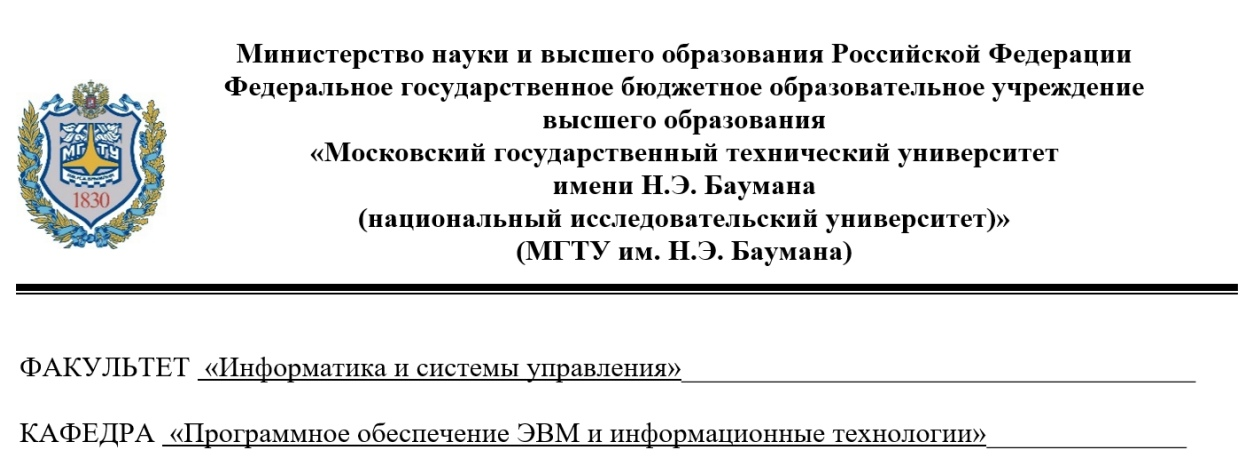
\includegraphics[scale = 0.4]{titul.jpg}}
			\label{titul}
		\end{center}
	\end{figure}
	
	\vspace*{15mm} 
	
	\huge
	\begin{center}
		Дисциплина: <<Моделирование>>
	\end{center}
	
	\begin{center}
		Лабораторная работа №4
	\end{center}

	
	\huge
	\begin{center}
		Тема работы:\\
		<<Программно- алгоритмическая реализация моделей на основе дифференциальных уравнений в частных производных с краевыми условиями II и  III рода.>>
	\end{center}
	\vspace*{25mm} 
	
	\large
	\begin{flushright}
		Студент: Левушкин И. К. \\
		Группа: ИУ7-62Б \\
		Преподаватель: Градов В. М. \\
	\end{flushright}
	
	\vspace*{25mm}
	\begin{center}
		Москва, 2020 г.  
	\end{center}
	\thispagestyle{empty}
	
	
	\newpage
	
	\section*{Цель работы}
	
	Получение навыков разработки  алгоритмов решения смешанной краевой задачи при реализации моделей, построенных на квазилинейном уравнении параболического типа.
	
	\section*{Исходные данные}
	
	\begin{enumerate}
		\item Задана математическая модель.
		
		Уравнение для функции $T(x, t)$
		
		\begin{equation}
		c(T) \frac{\partial T}{\partial t} = \frac{\partial}{\partial x} \left(k(T) \frac{\partial T}{\partial x}\right) - \frac{2}{R} \alpha(x) T + \frac{2 T_0}{R} \alpha(x) 
		\end{equation}
		
		Краевые условия
		
		\[
		\begin{cases}
		t = 0, T(x, 0) = T_0,
		
		x = 0, -k(T(0))\frac{\partial T}{\partial x} = F_0,\\
		
		x = l, -k(T(l))\frac{\partial T}{\partial x} = \alpha_N(T(l) - T_0)
		\end{cases}
		\]
		
		В обозначениях уравнения (14.1) лекции №14
		
		\[p(x) = \frac{2}{R} \alpha(x), f(u) \equiv f(x) = \frac{2 T_0}{R} \alpha(x).\]
		
		\item Разностная схема с разностным краевым условием при $x = 0$ получена в Лекции №14 (14.6),(14.7) и может быть использована в данной работе. Самостоятельно надо получить интегро-интерполяционным методом разностный аналог краевого условия при $x = l$, точно так же, как это сделано при $x = 0$ (формула (14.7)). Для этого надо проинтегрировать на отрезке $[x_{N-\frac{1}{2}}, x_N]$ выписанное выше уравнение (1) и учесть, что поток $\widehat{F_N} = \alpha_N (\widehat{y_N} - T_0)$, а $\widehat{F_{N - \frac{1}{2}}} = \widehat{\chi_{N - \frac{1}{2}}} \frac{\widehat{y_{N - 1}} - \widehat{y_N}}{h}$ .
		
		\item Значения параметров для отладки (все размерности согласованы)
		
		$k(T) = a_1 (b_1 + c_1 T^{m_1})$, Вт/см К,
		
		$c(T) = a_2 + b_2 T^{m_2} - \frac{c_2}{T^2}$, Дж/см$^3$ К.
		
		$a_1 = 0.0134, b_1 = 1, c_1 = 4.35 10^{-4}, m_1 = 1,$
		
		$a_2 = 2.049, b_2 = 0.563 10^{-3}, c_2 = 0.528 10^5, m_2 = 1.$
		
		$\alpha_0 = 0.05$ Вт/см$^2$ К,
		
		$\alpha_N = 0.01$ Вт/см$^2$ К,
		
		$l = 10$ см,
		
		$T_0 = 300$ К,
		
		$R = 0.5$ см,
		
		$F(t) = 50$ Вт/см$^2$ (для отладки принять постоянным)
	\end{enumerate}

	\section*{Физическое содержание задачи (для понимания получаемых результатов при отладке программы).}
	
	Постановки задач в данной лабораторной  работе и работе №3 во многом совпадают. Отличия заключаются в следующем:
	
	\begin{enumerate}
		\item Сформулированная в данной работе  математическая модель описывает {\bf нестационарное} температурное поле  $T(x, t)$, зависящее от координаты x и меняющееся во времени.
		\item Свойства материала стержня привязаны к температуре, т.е. теплоемкость и коэффициент теплопроводности $c(T), k(T)$ зависят от $T$, тогда как в работе №3 $k(x)$ зависит от координаты, а $c = 0$.  
		\item При $x = 0$ цилиндр нагружается тепловым потоком $F(t)$, в общем случае зависящим от времени, а в работе №3 поток был постоянный.
		
		Если в настоящей работе задать  поток постоянным, т.е. $F(t) = const$, то  будет происходить формирование температурного поля от начальной температуры $T_0$ до некоторого установившегося (стационарного) распределения $T(x, t)$. Это поле в дальнейшем с течением времени меняться не будет и должно совпасть с температурным распределением $T(x)$, получаемым в лаб. работе №3, если все параметры задач совпадают, в частности, вместо $k(T)$ надо использовать $k(x)$ из лаб. работы №3. Это полезный факт для тестирования программы.
		
		Если после разогрева стержня положить поток  $F(t) = 0$, то будет происходить остывание, пока температура не выровняется по всей длине и не станет равной $T_0$.
		
		При произвольной зависимости потока $F(t)$ от времени температурное поле будет как-то сложным образом отслеживать поток.
		
		\textit{Замечание.} Варьируя параметры задачи, следует обращать внимание на то, что решения, в которых температура превышает примерно 2000К, физического смысла не имеют и практического интереса не представляют.
	\end{enumerate}

	\section*{Результаты работы}
	
	\subsection*{Задание 1.}
	
	\textit{Представить разностный аналог краевого условия при $x = l$ и его краткий вывод интегро-интерполяционным методом.}
	
	Проинтегрируем уравнение (14.3) с учетом (14.2) из Лекции №14 на отрезке $[x_{N-\frac{1}{2}}, x_N]$ и на временном интервале $[t_m, t_{m+1}]$
	
	\begin{eqnarray} \int_{x_{N-\frac{1}{2}}}^{x_N}dx\int_{t_m}^{t_{m+1}}c(u)\frac{\partial u}{\partial t}dt = \nonumber \\ -\int_{t_m}^{t_{m+1}}dt\int_{x_{N-\frac{1}{2}}}^{x_N}\frac{\partial F}{\partial x}dx-\int_{x_{N-\frac{1}{2}}}^{x_N}dx\int_{t_m}^{t_{m+1}}p(x)u dt+\int_{x_{N-\frac{1}{2}}}^{x_N}\int_{t_m}^{t_{m+1}}f(u)dt \nonumber
	\end{eqnarray}
	
	Приближенно вычисляя итегралы по времени, как и выше получим
	
	\[\int_{x_{N-\frac{1}{2}}}^{x_N}\widehat{c}(\widehat{u}-u)dx = 
	-\int_{t_m}^{t_{m+1}}(F_N-F_{N-\frac{1}{2}})dt-\int_{x_{N-\frac{1}{2}}}^{x_N}p\widehat{u}\tau dx + \int_{x_{N-\frac{1}{2}}}^{x_N}\widehat{f}\tau dx\]
	
	Вычисляем интегралы. Первый интеграл справа, как и ранее, находим методом
	правых прямоугольников, а остальные - методом трапеций
	
	\begin{eqnarray}
	\frac{h}{4}\left[\widehat{c_N}(\widehat{y_N}-y_N)+\widehat{c_{N-\frac{1}{2}}}(\widehat{y_{N-\frac{1}{2}}} - y_{N-\frac{1}{2}}) \right] = \nonumber \\ -(\widehat{F_N} - \widehat{F_{N - \frac{1}{2}}})\tau - (p_N\widehat{y_N} + p_{N-\frac{1}{2}}\widehat{y_{N-\frac{1}{2}}})\tau \frac{h}{4} + (\widehat{f_{N - \frac{1}{2}}} + \widehat{f_N})\tau \frac{h}{4} \nonumber
	\end{eqnarray}
	
	Подставляя в данное уравнение выражение для потока $\widehat{F_{N - \frac{1}{2}}}$, учитывая, что $\widehat{F_N} = F(t_{m + 1}) = \alpha (\widehat{y_N} - \beta)$ (где $\alpha = \alpha_N, \beta = T_0$), и заменяя $\widehat{y_{N - \frac{1}{2}}} = \frac{\widehat{y_N} + \widehat{y_{N - 1}}}{2}, y_{N - \frac{1}{2}} = \frac{y_N + y_{N - 1}}{2}$, найдем разностный аналог краевого условия
	
	\begin{eqnarray}
	\left[
	\alpha \tau + \frac{h}{4} \widehat{c_N} + \frac{h}{8} \widehat{c_{N - \frac{1}{2}}} + \frac{\widehat{\chi_{N - \frac{1}{2}}} \tau}{h} + \frac{p_N \tau h}{4} + \frac{p_{N - \frac{1}{2}} \tau h}{8}
	\right] \widehat{y_N} +\nonumber\\ 
	\left[
	\frac{h}{8}\widehat{c_{N - \frac{1}{2}}} - \frac{\widehat{\chi_{N - \frac{1}{2}}} \tau}{h} + \frac{p_{N - \frac{1}{2}} \tau h}{8}
	\right] \widehat{y_{N-1}} =\nonumber\\
	\alpha \beta \tau + (\widehat{f_{N - \frac{1}{2}}} + \widehat{f_N})\tau \frac{h}{4} + \frac{h}{4} \widehat{c_N} y_N + \frac{h}{4} \widehat{c_{N - \frac{1}{2}}} \frac{y_N + y_{N - 1}}{2}\nonumber
	\end{eqnarray}
	
	
	
	\newpage
	
	\subsection*{Задание 2.}
	
	\textit{График зависимости температуры $T(x, t_m)$ от координаты $x$ при нескольких фиксированных значениях времени $t_m$ (аналогично рисунку в лекции №14) при заданных выше параметрах. Обязательно представить распределение $T(x, t)$ в момент времени, соответствующий установившемуся режиму, когда поле перестает меняться с некоторой точностью (например, $\left[\frac{T(t + \tau) - T(t)}{T(t + \tau)}\right] < 10^{-4}$), т.е. имеет место выход на стационарный режим. На этой стадии левая часть дифференциального уравнения близка к нулю, и на самом деле решается уравнение из лабораторной работы №3 (отличие только в том, что там было линейное уравнение).}
	
	
	Ниже приведены графики зависимости температуры стержня $T$, зависящее от координаты $x$ в разные моменты времени $t_m$ - от начального момента $t = 0$ (синий график) до момента, когда поле перестает меняться с точностью (серый график): $\left[\frac{T(t + \tau) - T(t)}{T(t + \tau)}\right] < 10^{-4}$. Поток постоянный: $F(x) = const = F_0$. Шаг по $x$: $h_x = 0.01$ см. Шаг по $t$: $h_t = 1$ сек.. Все остальные параметры взяты из значений параметров для отладки.
	
	
	\begin{figure}[h!]
		\begin{center}
			{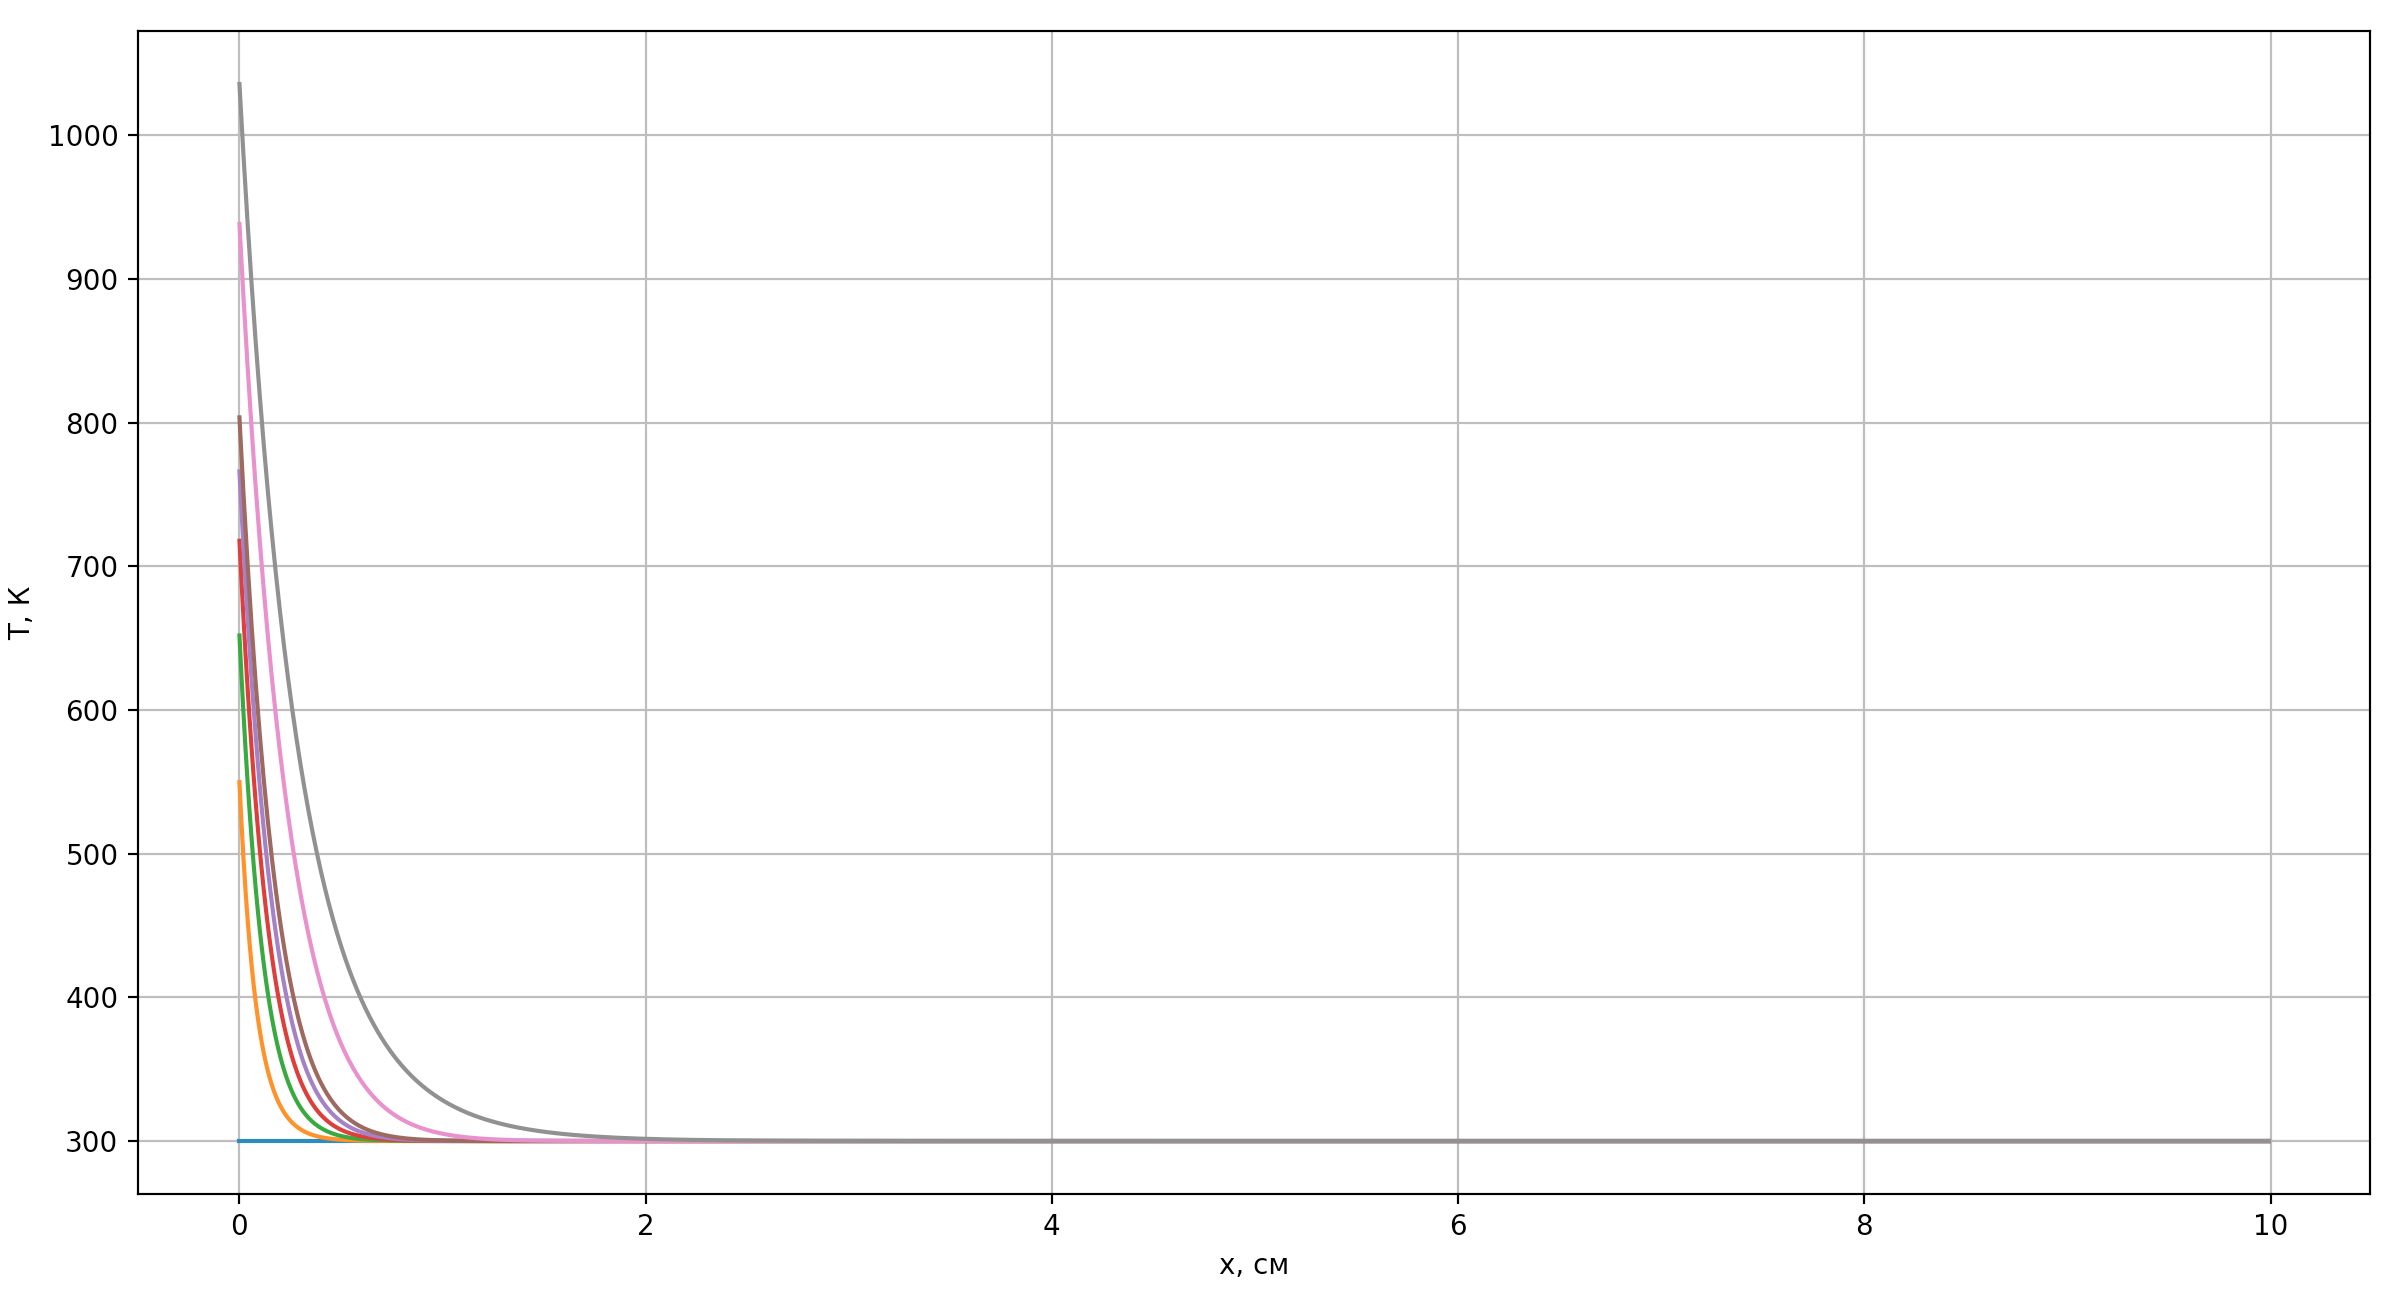
\includegraphics[scale = 0.4]{1.png}}
			\label{ris:1}
		\end{center}
		\caption{Графики зависимости температуры $T(x, t_m)$ при $h_x$ = 0.01 см; $h_t = 1$ сек.; $F_0 = 50.0$ Вт/см$^2$.}
	\end{figure}
	
	\newpage
	
	\begin{figure}[h!]
		\begin{center}
			{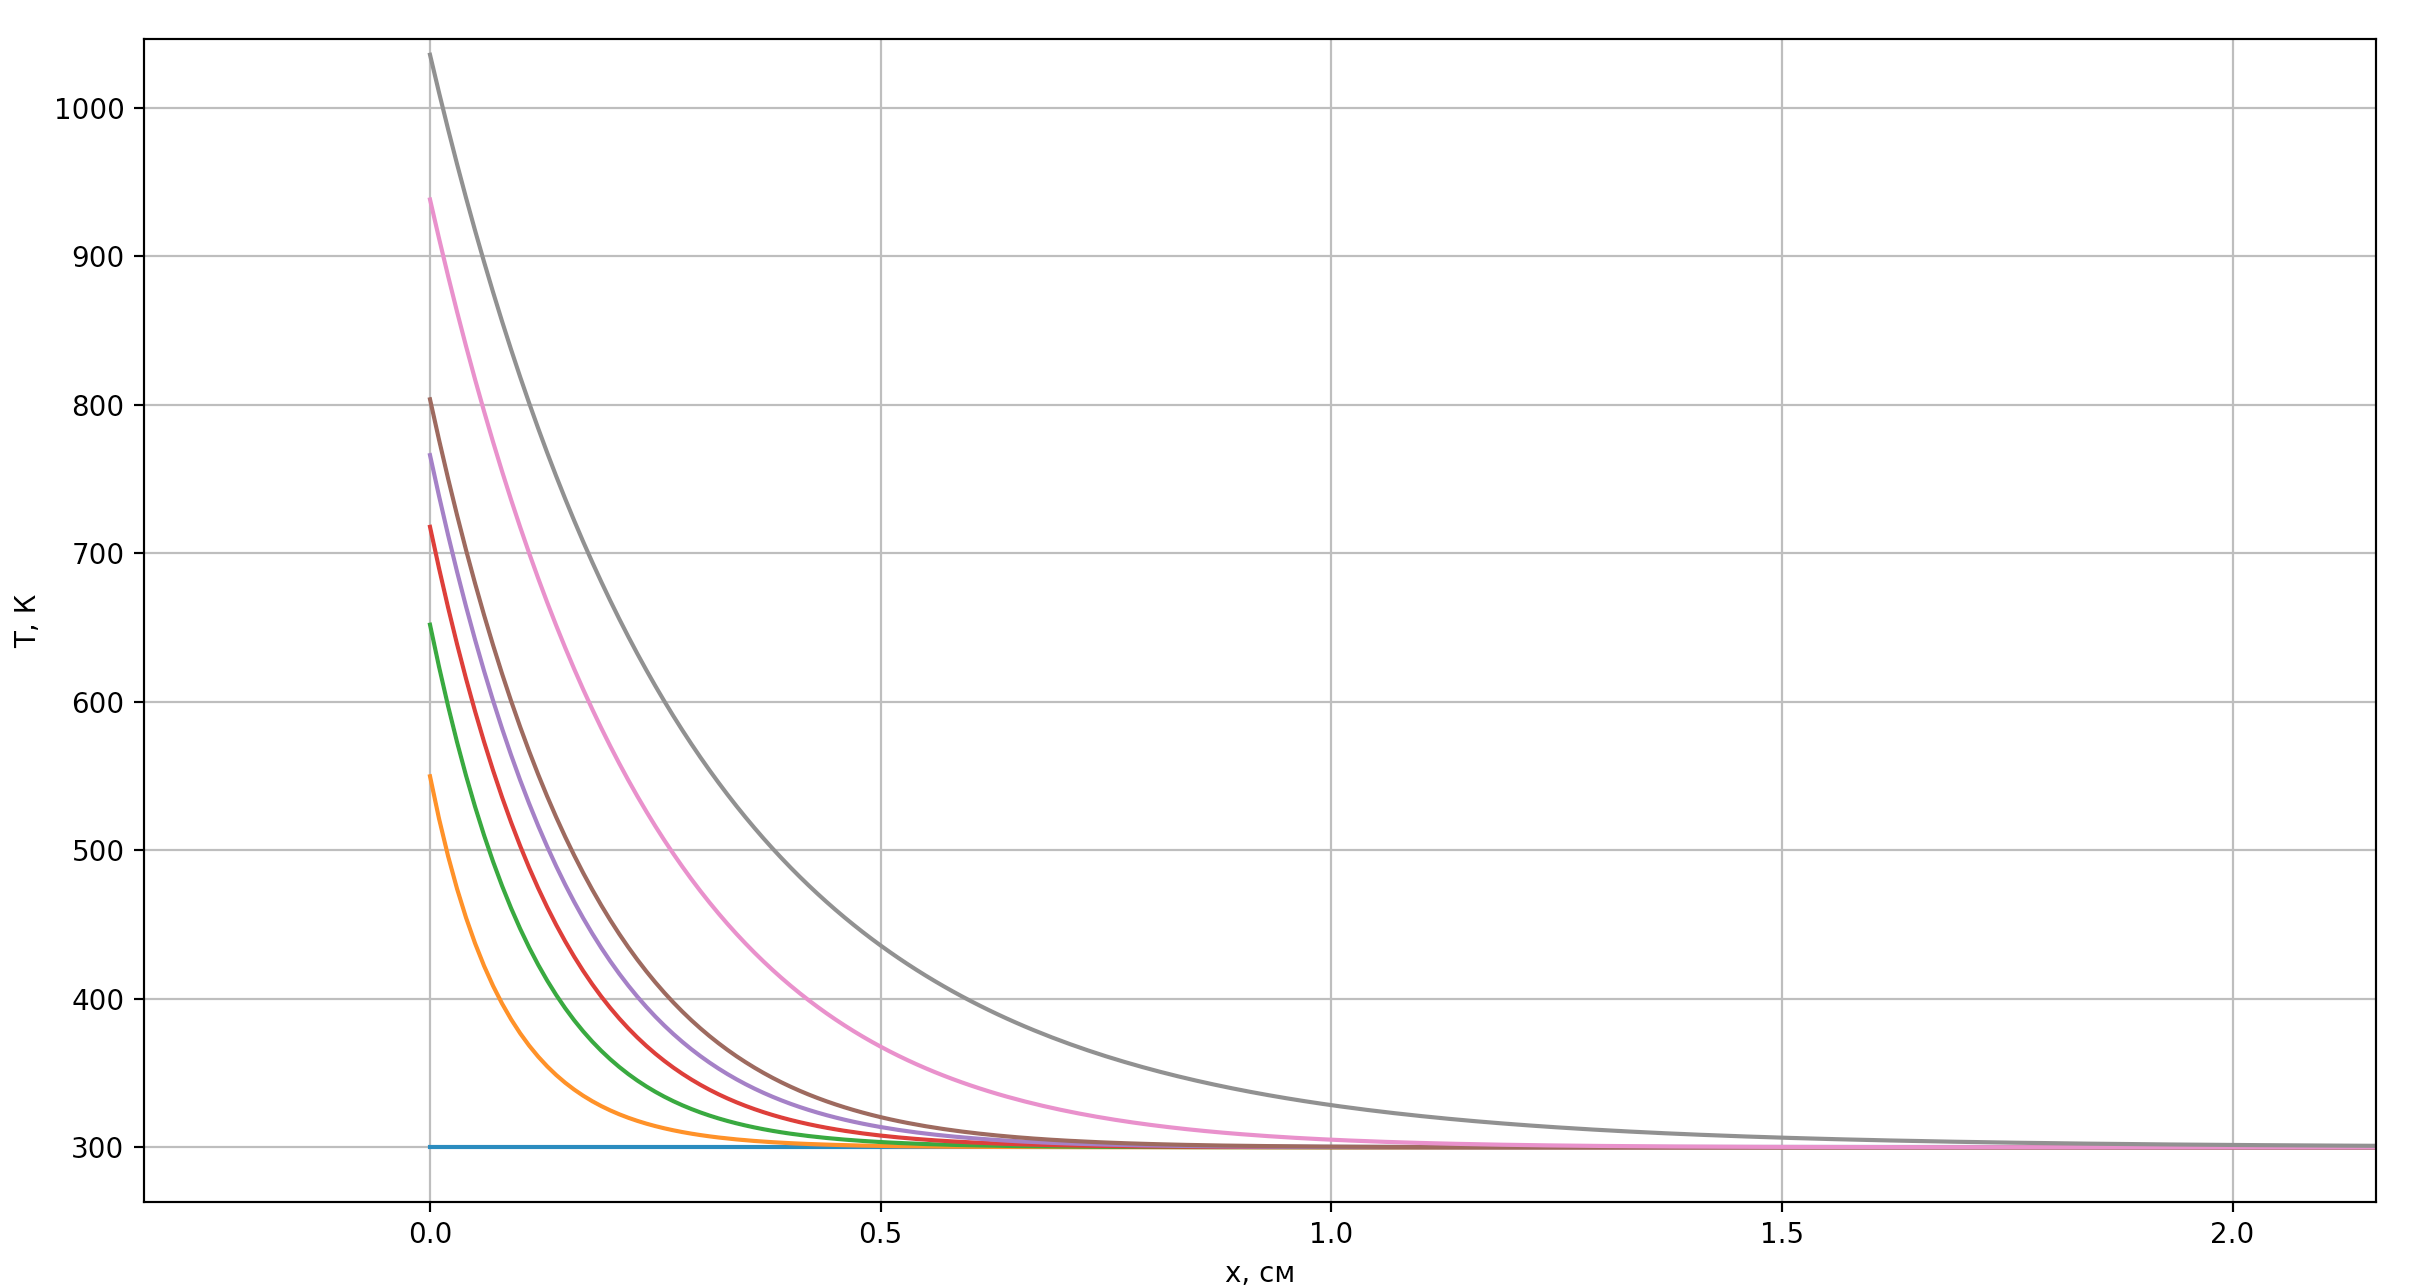
\includegraphics[scale = 0.4]{2.png}}
			\label{ris:2}
		\end{center}
		\caption{Графики зависимости температуры $T(x, t_m)$ при $h_x$ = 0.01 см; $h_t = 1$ сек.; $F_0 = 50.0$ Вт/см$^2$.}
	\end{figure}

	Где 
	\begin{itemize}
		\item Синий цвет соответствует графику при $t = 0$ сек..
		\item Оранжевый цвет соответствует графику при $t = 1$ сек..
		\item Зеленый цвет соответствует графику при $t = 2$ сек..
		\item Красный цвет соответствует графику при $t = 3$ сек..
		\item Фиолетовый цвет соответствует графику при $t = 4$ сек..
		\item Коричневый цвет соответствует графику при $t = 5$ сек..
		\item Розовый цвет соответствует графику при $t = 12$ сек..
		\item Серый цвет соответствует графику при $t = 71$ сек. (стационарный режим).
	\end{itemize}
	\newpage
	
	\subsection*{Задание 3.}
	
	 \textit{График зависимости $T(x_n, t)$ при нескольких фиксированных значениях координаты $x_n$. Обязательно представить случай $n = 0$, т.е. $x = x_0 = 0$.}
	 
	 Ниже приведены графики зависимости температуры стержня T от координаты t в разные моменты времени $x_n$ - от начала стержня $x = 0.0$ см (синий график) до конца стержня $x = 10.0$ (серый график). Поток постоянный: $F(x) = const = F_0$. Шаг по $x$: $h_x = 0.01$ см. Шаг по $t$: $h_t = 1$ сек.. Все остальные параметры взяты из значений параметров для отладки.
	 
	 \begin{figure}[h!]
	 	\begin{center}
	 		{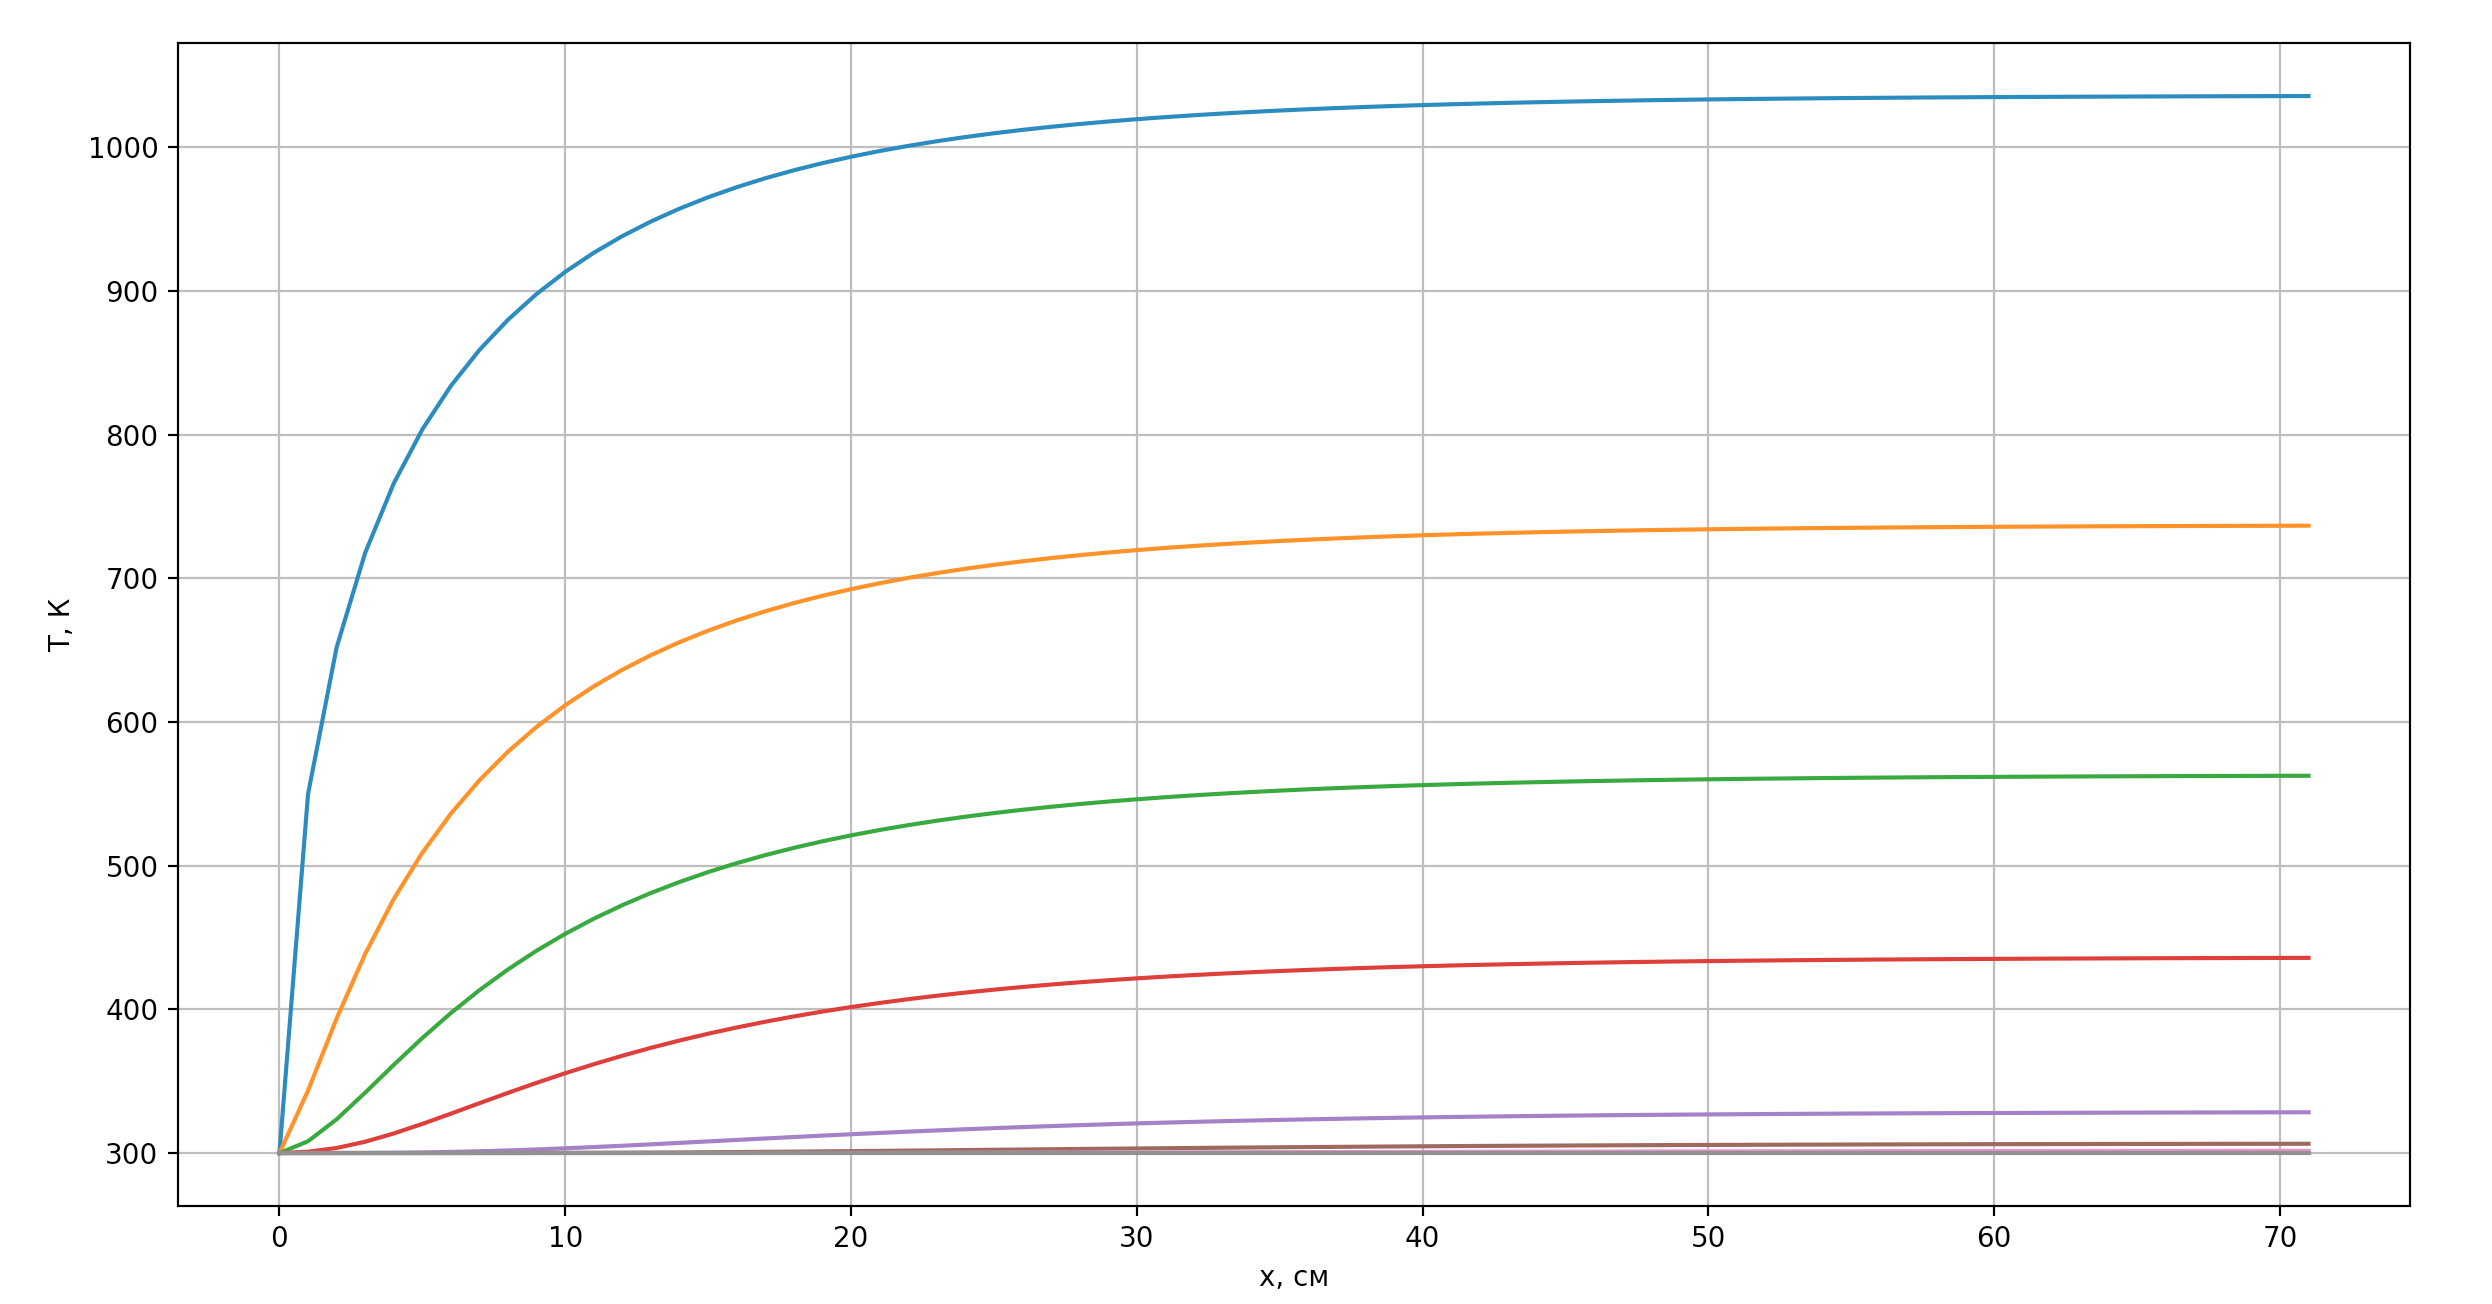
\includegraphics[scale = 0.4]{8.png}}
	 		\label{ris:8}
	 	\end{center}
	 	\caption{Графики зависимости температуры $T(x_n, t)$ при $h_x$ = 0.01 см; $h_t = 1$ сек.; $F_0 = 50.0$ Вт/см$^2$.}
	 \end{figure}
	 
	 \linebreak Где 
	 \begin{itemize}
		\item Синий цвет соответствует графику при $x = 0$ см.
		\item Оранжевый цвет соответствует графику при $x = 0.15$ см.
		\item Зеленый цвет соответствует графику при $x = 0.3$ см.
		\item Красный цвет соответствует графику при $x = 0.5$ см.
		\item Фиолетовый цвет соответствует графику при $x = 1.0$ см.
		\item Коричневый цвет соответствует графику при $x = 1.5$ см.
		\item Розовый цвет соответствует графику при $x = 2.0$ см.
		\item Серый цвет соответствует графику при $x = 10.0$ см.
	 \end{itemize}
	 
	 \section*{Вопросы при защите лабораторной работы.}
	 
	 \textit{Ответы на вопросы дать письменно в Отчете о лабораторной работе.}
	 
	 \subsection*{1. Приведите результаты тестирования программы (графики, общие соображения, качественный анализ). Учесть опыт выполнения лабораторной работы №3.}
 	
 	\subsubsection*{Пример 1.}
 	
 	Ниже приведены графики зависимости температуры стержня $T$, зависящее от координаты $x$ в разные моменты времени $t_m$ - от начального момента $t = 0$ (синий график) до момента, когда поле перестает меняться с точностью (серый график): $\left[\frac{T(t + \tau) - T(t)}{T(t + \tau)}\right] < 10^{-4}$. Поток постоянный: $F(x) = const = F_0$. Шаг по $x$: $h_x = 0.01$ см. Шаг по $t$: $h_t = 1$ сек.. Все остальные параметры взяты из значений параметров для отладки за исключением $k(T)$ (заменен на $k(x)$ из лаб. работы №3). 
 	\newpage
 	\begin{figure}[h!]
 		\begin{center}
 			{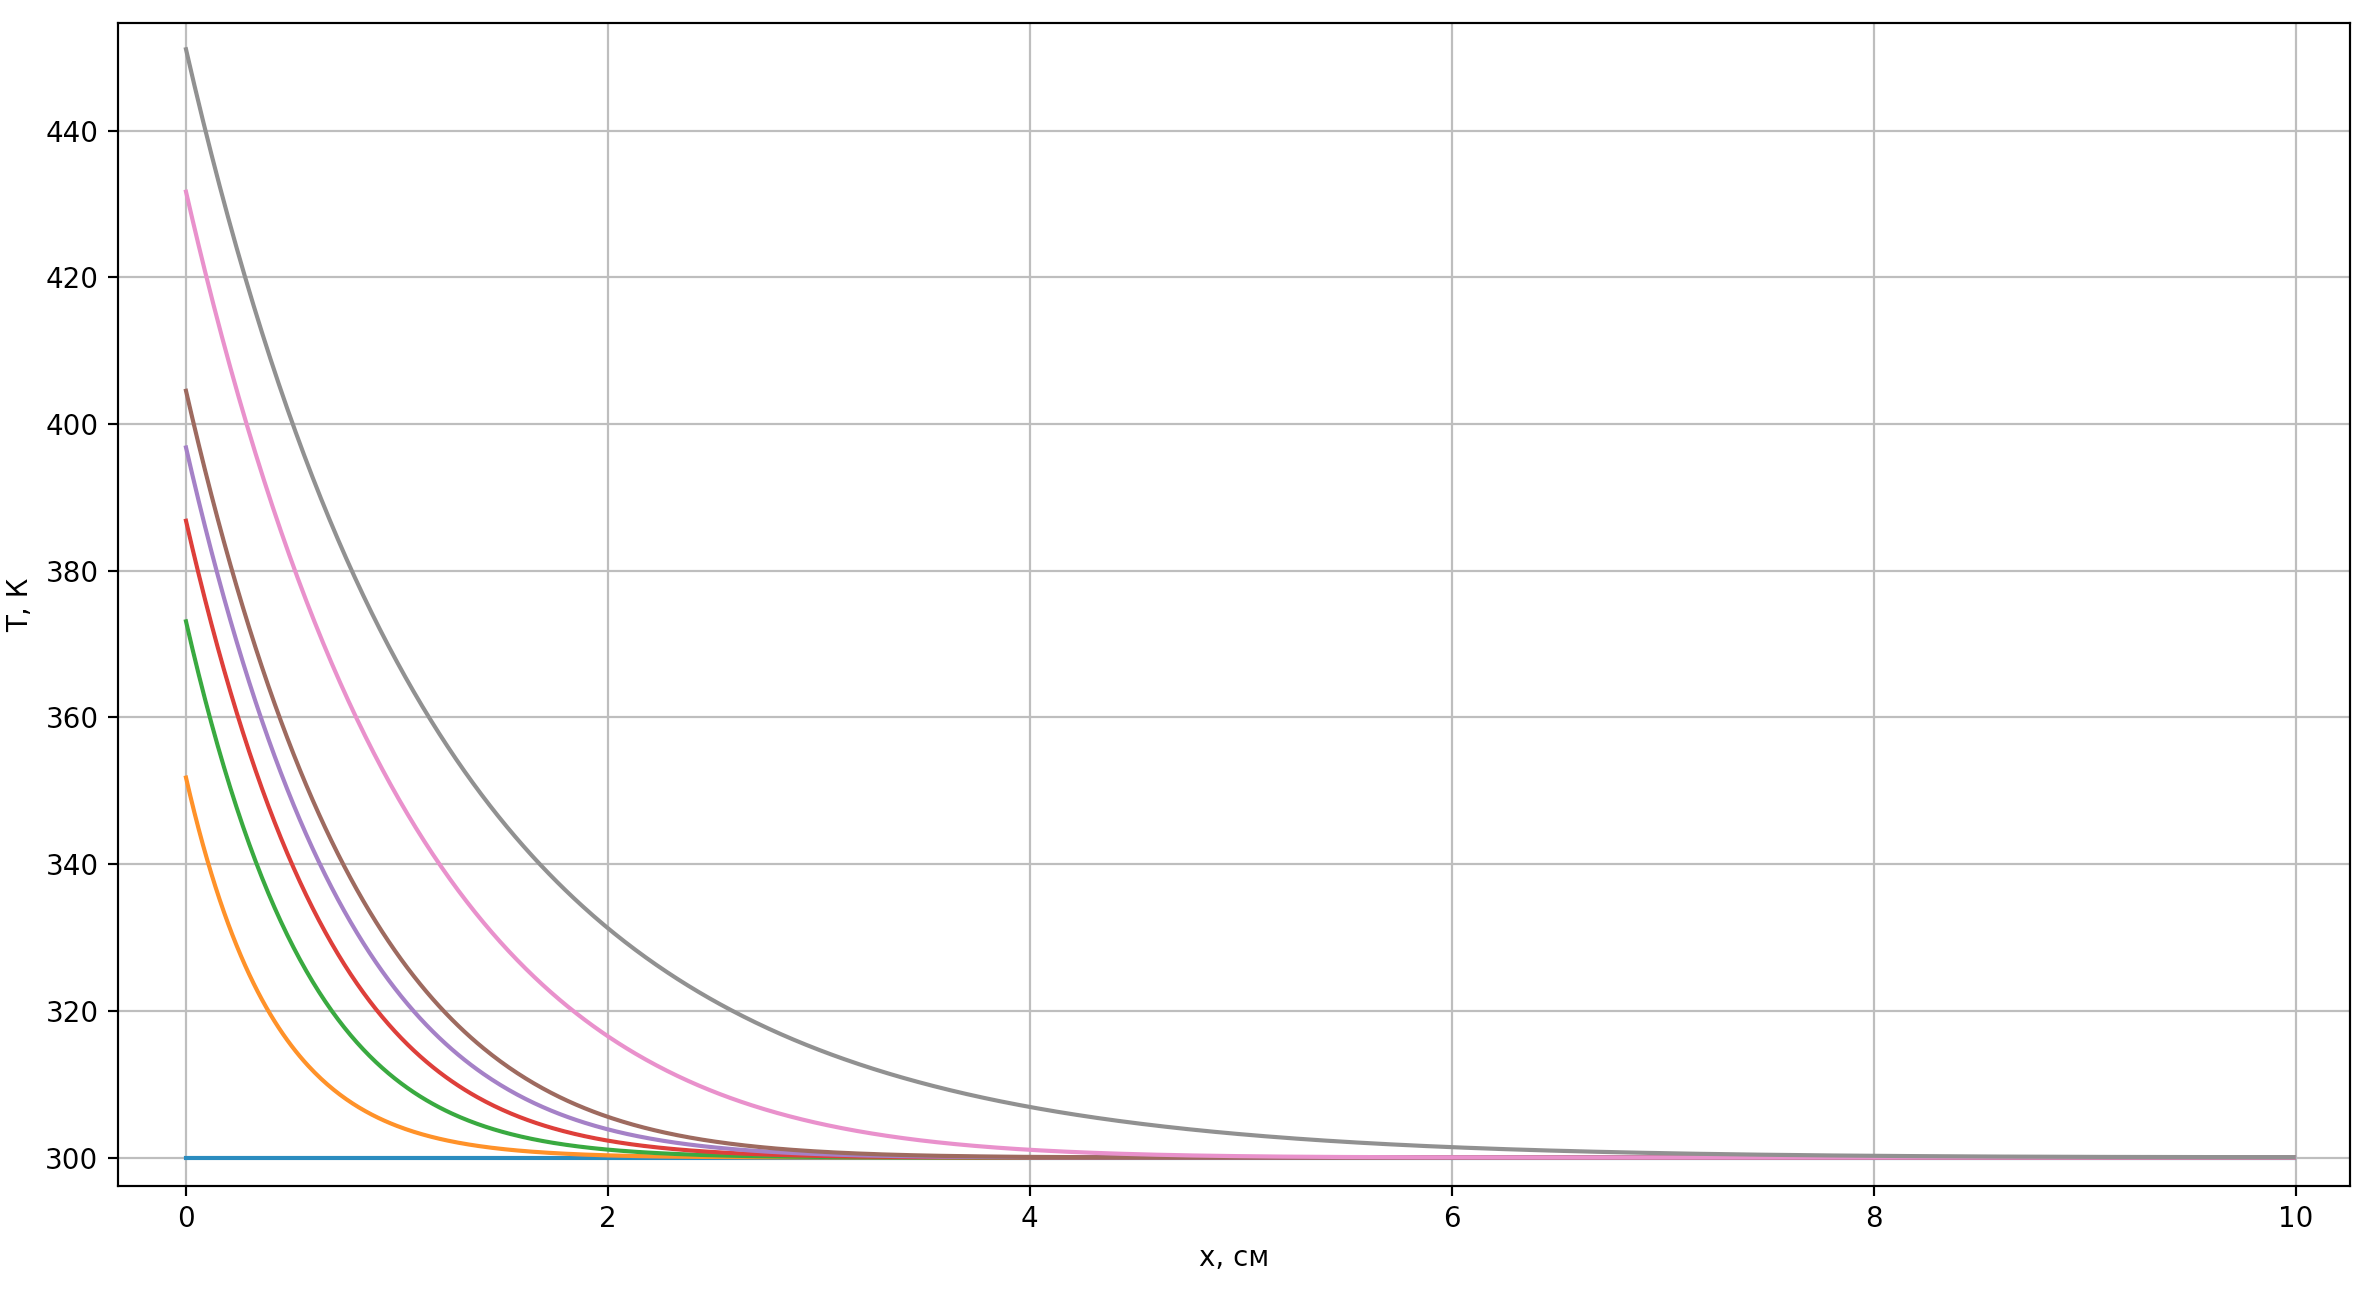
\includegraphics[scale = 0.4]{3.png}}
 			\label{ris:3}
 		\end{center}
 		\caption{Графики зависимости температуры $T(x, t_m)$ при $h_x$ = 0.01 см; $h_t = 1$ сек.; $F_0 = 50.0$ Вт/см$^2$.}
 	\end{figure}
 
 	\linebreak Где график серого цвета отвечает за состояние температуры стержня в момент установления стационарного режима. Этот график полностью совпадает с графиком, полученным в 3 лаб. работе при тех же параметрах, что иллюстрирует правильную работу программы.
 	
 	\newpage
 	
 	\subsubsection*{Пример 2.}
 	
 	Ниже приведены графики с теми же параметрами, что и в задании 2 из раздела <<Результаты работы>> за исключением $F(x) = const - 0.0$ Вт/см$^2$ и начальной температуры стержня. Она задается такой, какой была температура стержня из примера 1 в момент установления стационарного режима. Таким образом модулируется процесс остывания стержня после его разогрева.
 	
 	\begin{figure}[h!]
 		\begin{center}
 			{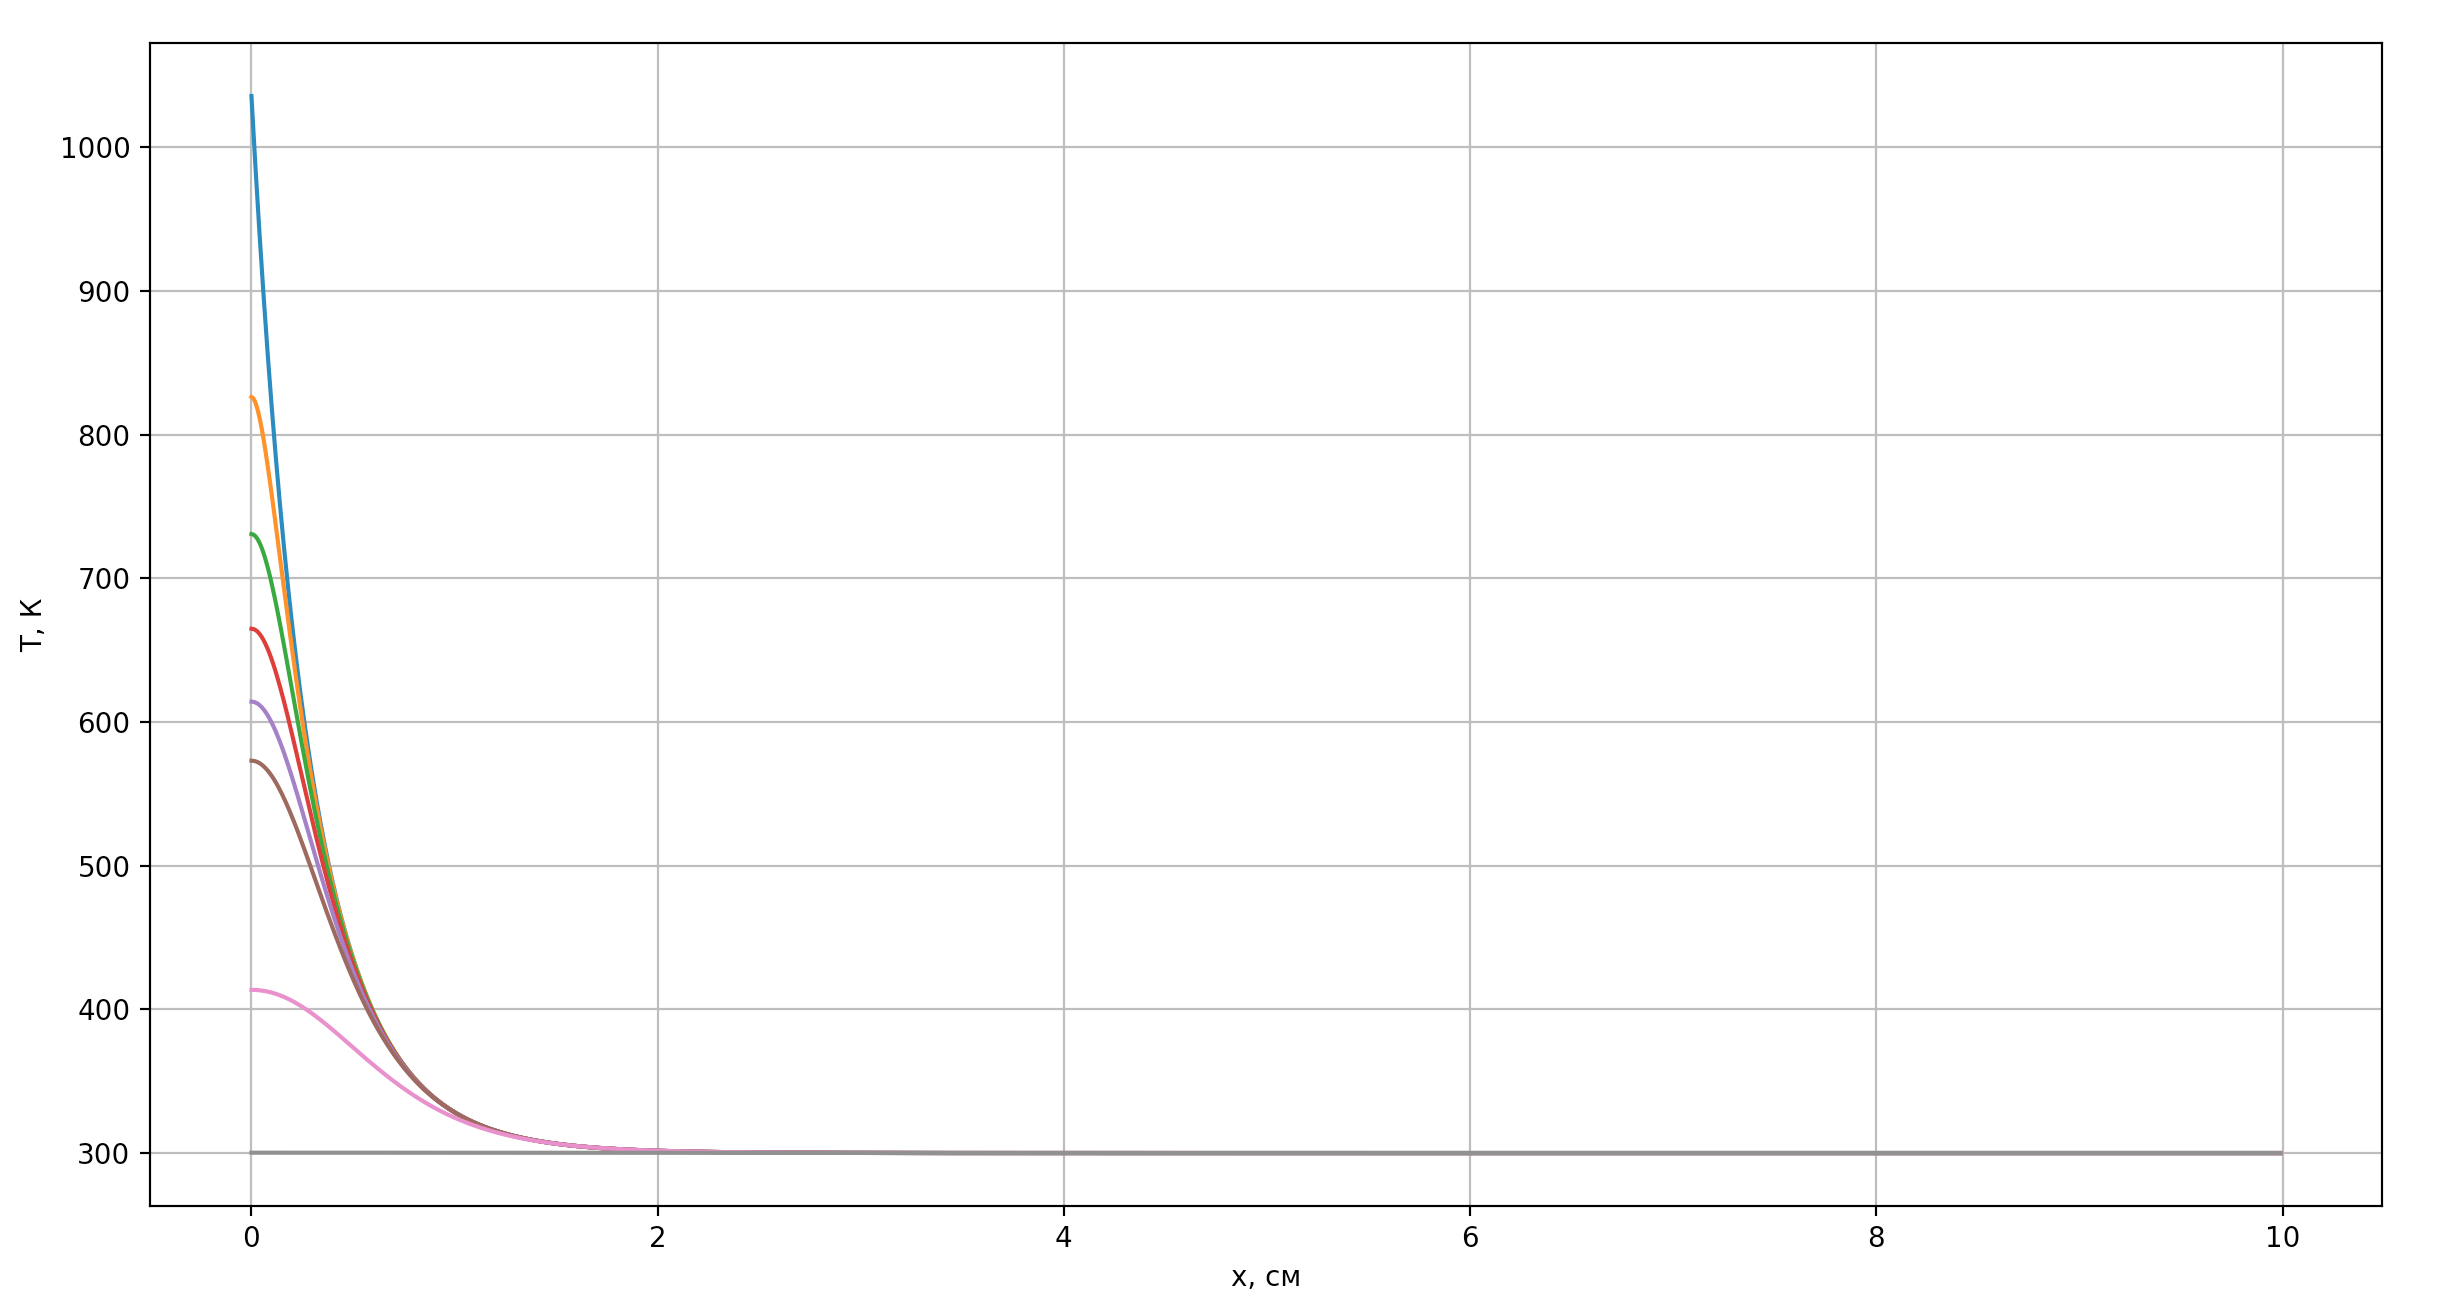
\includegraphics[scale = 0.4]{4.png}}
 			\label{ris:4}
 		\end{center}
 		\caption{Графики зависимости температуры $T(x, t_m)$ при $h_x$ = 0.01 см; $h_t = 1$ сек.; $F_0 = 0.0$ Вт/см$^2$.}
 	\end{figure}
 
 	\newpage
 
 	\begin{figure}[h!]
 		\begin{center}
 			{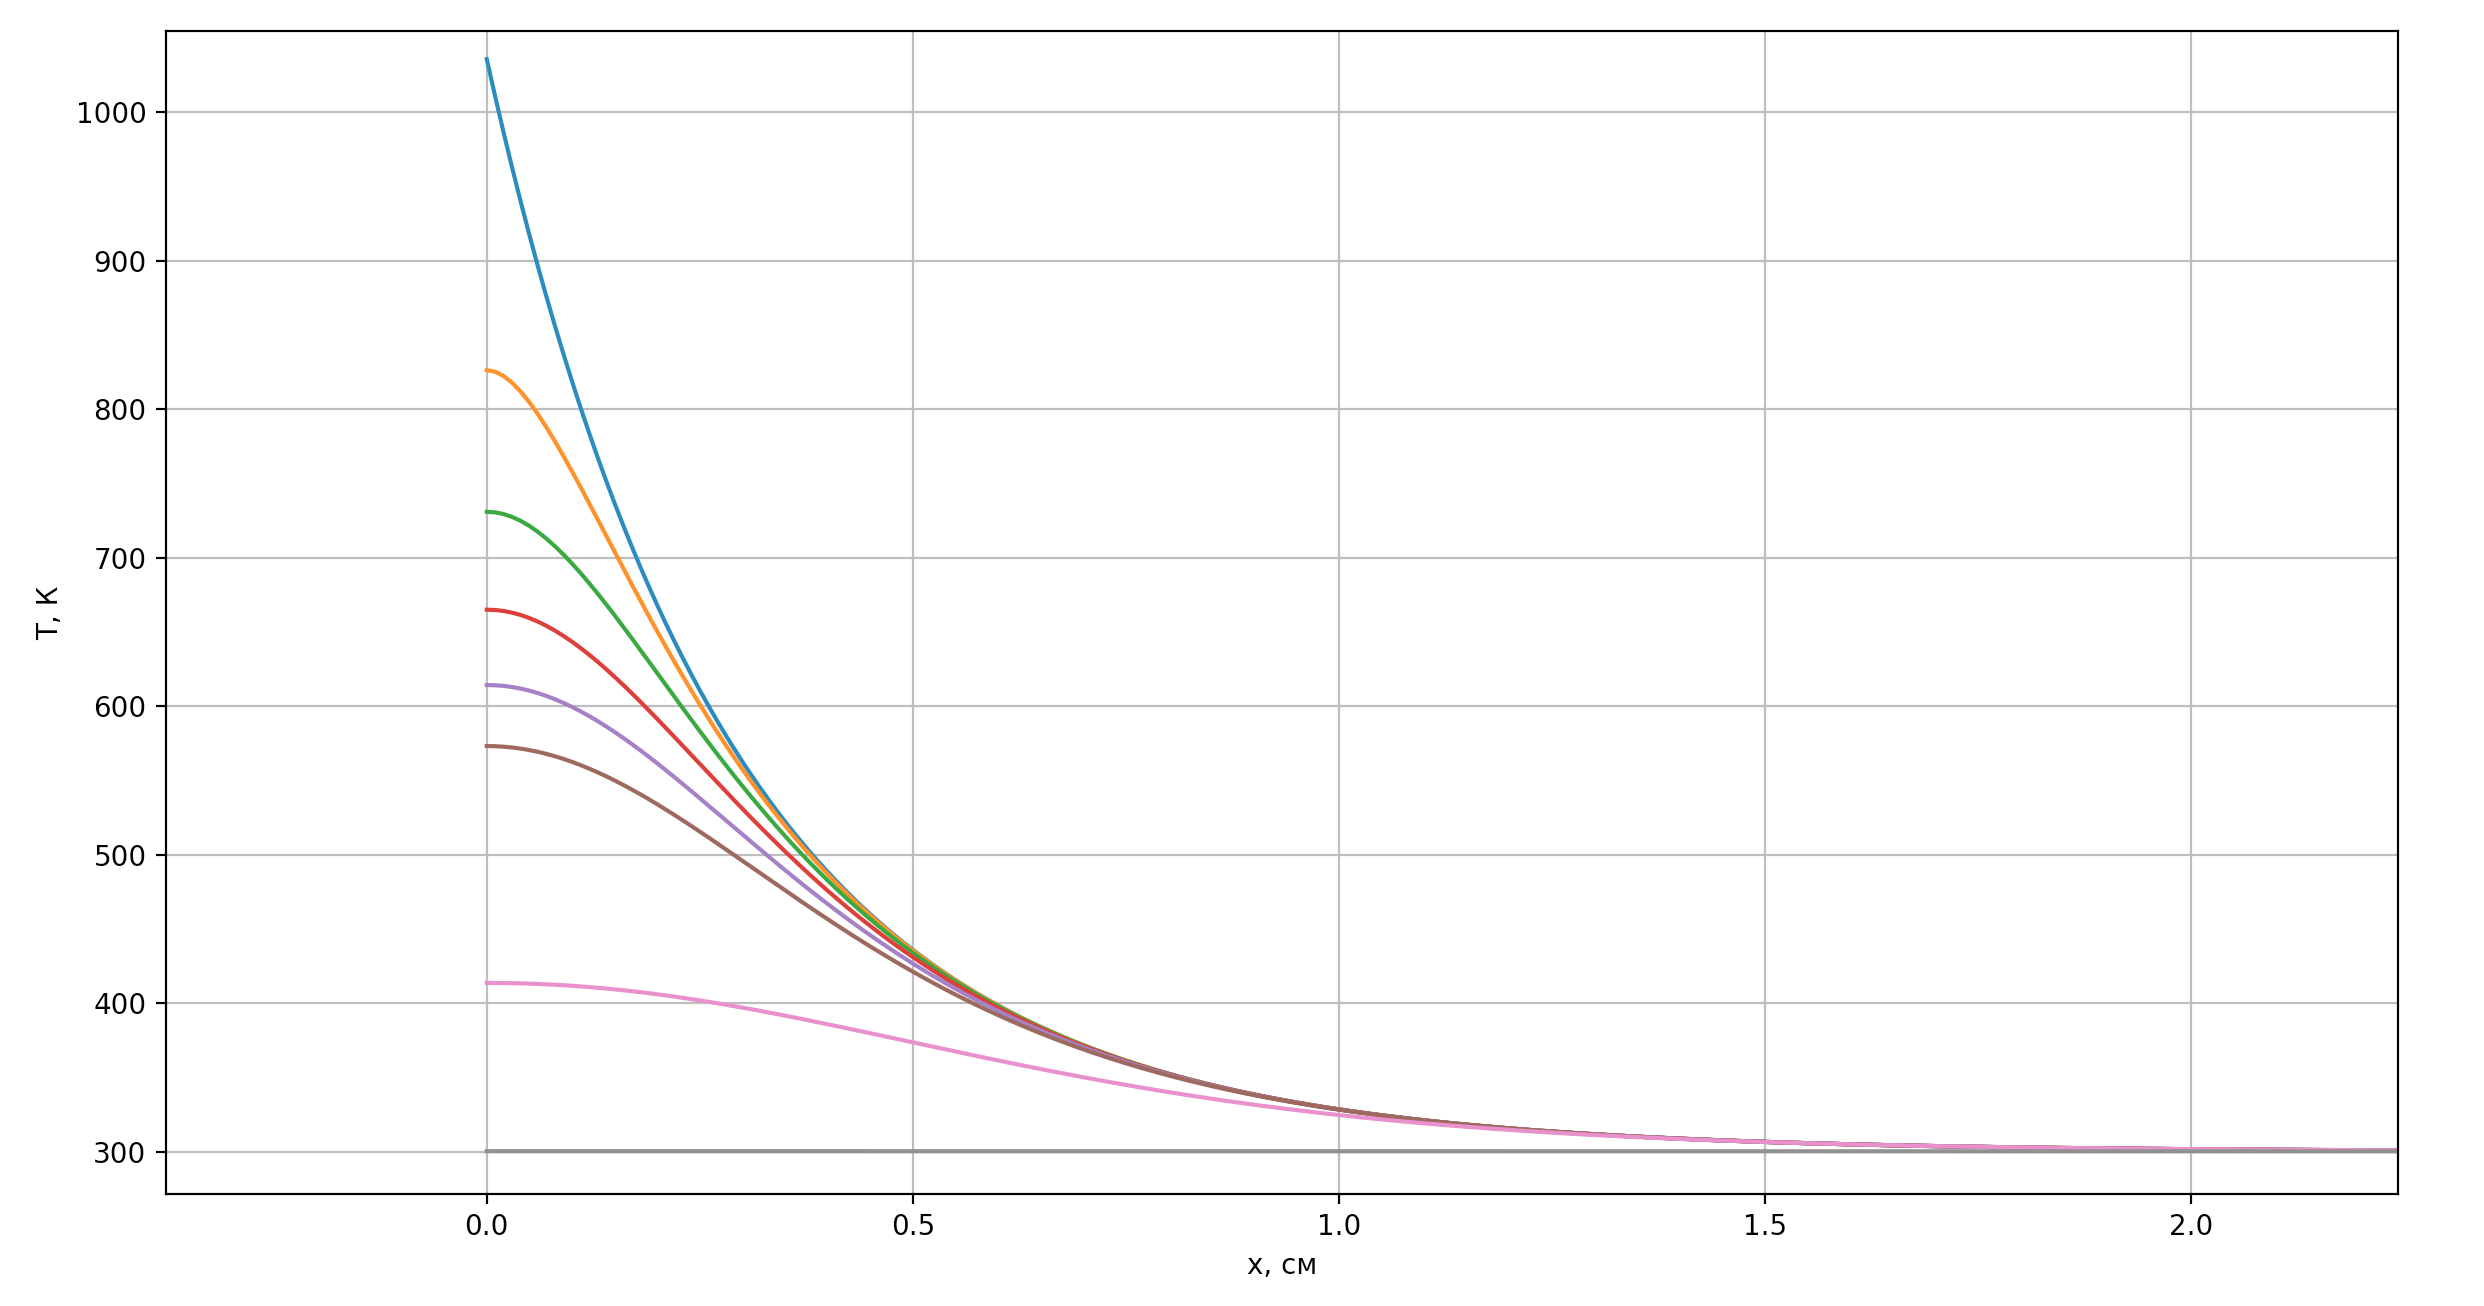
\includegraphics[scale = 0.4]{6.png}}
 			\label{ris:6}
 		\end{center}
 		\caption{Графики зависимости температуры $T(x, t_m)$ при $h_x$ = 0.01 см; $h_t = 1$ сек.; $F_0 = 0.0$ Вт/см$^2$.}
 	\end{figure}
 
 	\linebreak Где график серового цвета отвечает за состояние температуры стержня в момент установления стационарного режима. На нем, как и ожидалось, температура выровнилась по всей длине стержня и стала равной $T_0$, что также иллюстрирует правильную работу программы.
 
 	\newpage
 	
 	\subsubsection*{Пример 3.}
 	
 	Ниже приведены графики с теми же параметрами, что и в задании 2 из раздела <<Результаты работы>> за исключением того, что $F(t) \neq const$. Было решено задать $F(t) = 10 + 20 sin(t)$ Вт/см$^2$.
 	
 	\begin{figure}[h!]
 		\begin{center}
 			{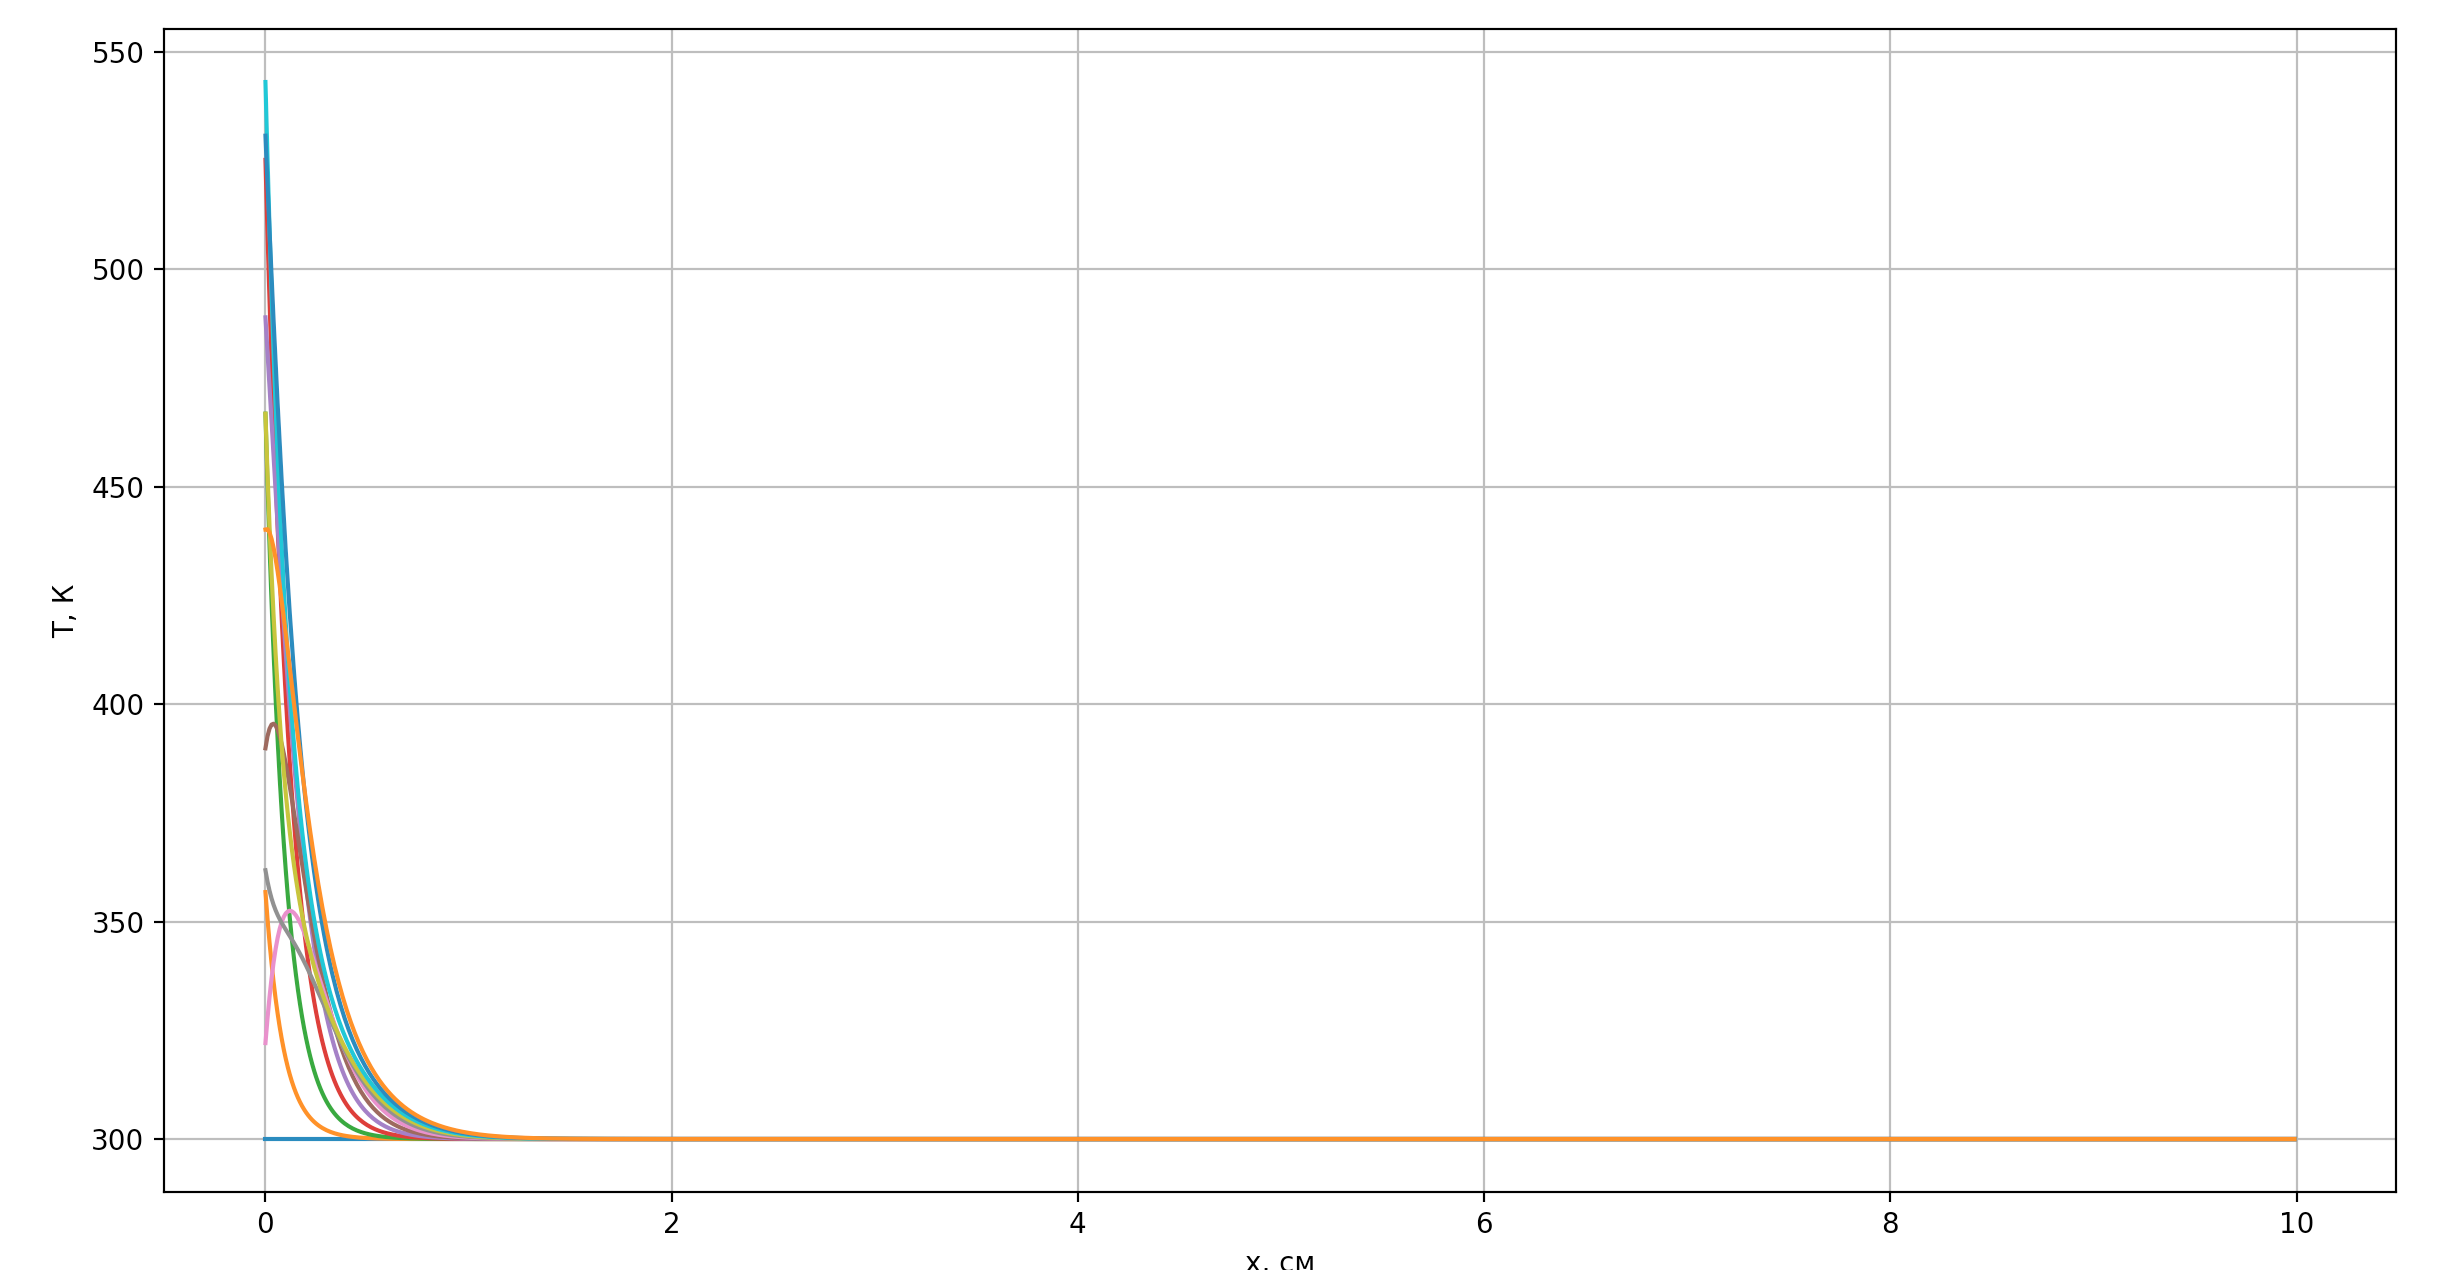
\includegraphics[scale = 0.4]{5.png}}
 			\label{ris:5}
 		\end{center}
 		\caption{Графики зависимости температуры $T(x, t_m)$ при $h_x$ = 0.01 см; $h_t = 1$ сек.; $F(t) = 10 + 20 sin(t)$ Вт/см$^2$.}
 	\end{figure}
 
 	\newpage
 	
 	\begin{figure}[h!]
 		\begin{center}
 			{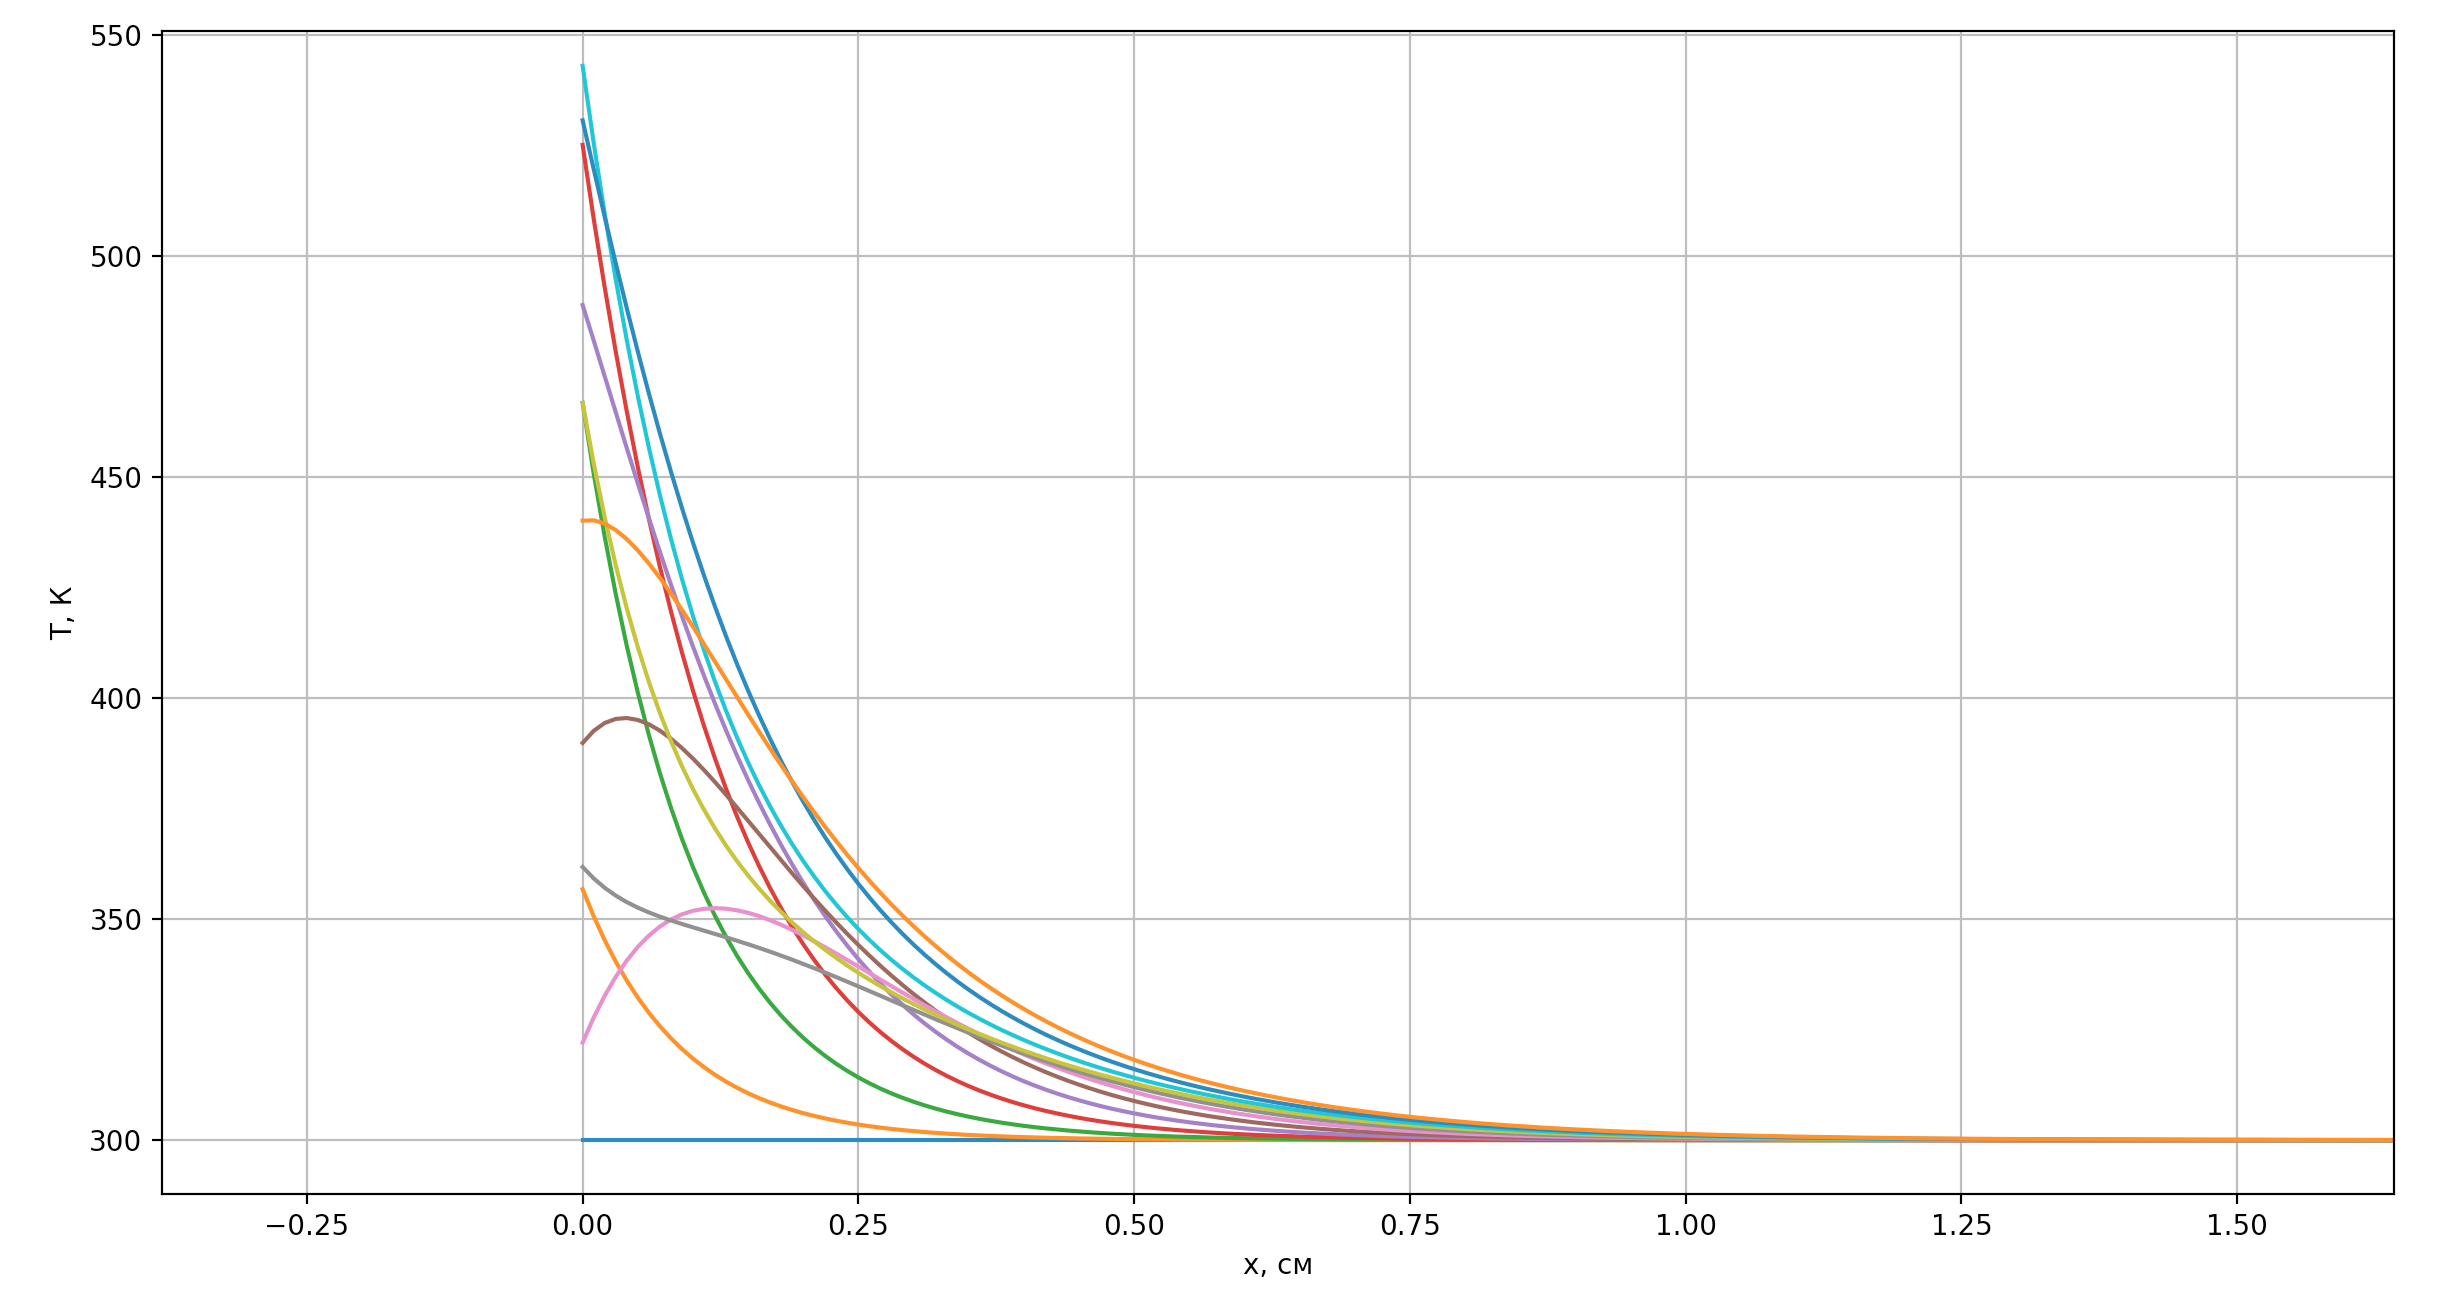
\includegraphics[scale = 0.4]{7.png}}
 			\label{ris:7}
 		\end{center}
 		\caption{Графики зависимости температуры $T(x, t_m)$ при $h_x$ = 0.01 см; $h_t = 1$ сек.; $F(t) = 10 + 20 sin(t)$ Вт/см$^2$.}
 	\end{figure}
 	
 	\linebreak Из графиков видно, что стержень то остывает, то нагревается в разные промежутки времени. Это происходит из-за немонотонности функции $F(t)$.
 
 	\newpage
 
	 \subsection*{2. Выполните линеаризацию уравнения (14.8) по Ньютону, полагая для простоты, что все коэффициенты зависят только от одной переменной $\widehat{y_n}$. Приведите линеаризованный вариант уравнения и опишите алгоритм его решения. Воспользуйтесь процедурой вывода, описанной в лекции №8.}
	
	В нащем случае:
	
	\[
	\widehat{A_n} = \widehat{A_n}(\widehat{y_n}), \widehat{B_n} = \widehat{B_n}(\widehat{y_n}), \widehat{C_n} = \widehat{C_n}(\widehat{y_n}), \widehat{D_n} = \widehat{D_n}(\widehat{y_n}).
	\]
	
	Выполняя линеаризацию по Ньютону по неизвестному $\widehat{y_n}$, получим
	
	\begin{eqnarray}
	(\widehat{A_n}\widehat{y_{n - 1}} - \widehat{B_n}\widehat{y_{n}}  + \widehat{D_n}\widehat{y_{n + 1}} + \widehat{F_n})|_{s-1} + \nonumber \\
	\frac{\delta (\widehat{A_n}\widehat{y_{n - 1}} - \widehat{B_n}\widehat{y_n}) + \widehat{D_n}\widehat{y_{n + 1}} + \widehat{F_n}}{\delta \widehat{y_{n - 1}}}|_{s-1} \Delta \widehat{y_{n - 1}^s} + \nonumber \\
	\frac{\delta (\widehat{A_n}\widehat{y_{n - 1}} - \widehat{B_n}\widehat{y_n}) + \widehat{D_n}\widehat{y_{n + 1}} + \widehat{F_n}}{\delta \widehat{y_{n}}}|_{s-1} \Delta \widehat{y_{n}^s} +  \nonumber \\
	\frac{\delta (\widehat{A_n}\widehat{y_{n - 1}} - \widehat{B_n}\widehat{y_n}) + \widehat{D_n}\widehat{y_{n + 1}} + \widehat{F_n}}{\delta \widehat{y_{n + 1}}}|_{s-1} \Delta \widehat{y_{n + 1}^s} = 0
	\end{eqnarray}
	
	\begin{eqnarray}
	(\widehat{A_n}\widehat{y_{n - 1}} - \widehat{B_n}\widehat{y_{n}}  + \widehat{D_n}\widehat{y_{n + 1}} + \widehat{F_n})|_{s-1} + \widehat{A_n}|_{s-1}\Delta \widehat{y_{n - 1}^s} + \nonumber \\
	\left(
	\frac{\delta \widehat{A_n}}{\delta \widehat{y_n}} \widehat{y_{n - 1}} - \frac{\delta \widehat{B_n}}{\delta \widehat{y_n}}\widehat{y_n} - \widehat{B_n} + \frac{\delta \widehat{D_n}}{\delta \widehat{y_n}}\widehat{y_{n + 1}} + \frac{\delta \widehat{F_n}}{\delta \widehat{y_n}}\right)|_{s - 1}\Delta \widehat{y_n^s} + \widehat{D_n}|_{s - 1} \Delta \widehat{y_{n + 1}^s} = 0
	\end{eqnarray}
	
	Уравнение (3) решается методом прогонки, в результате находитятся все $\Delta \widehat{y_n^s}$, после чего определяются значения искомой функции в узлах на s-итерации $\widehat{y_n^s} = \widehat{y_n^{s-1}} \Delta \widehat{y_n^s}$. Итерационный процесс заканчивается при выполнении условия $max\left|\frac{\Delta \widehat{y_n^s}}{\widehat{y_n^s}}\right| \leqslant \varepsilon$, для всех $n = 0,1,... N$
	
	\section*{Листинг кода программы}
	
	\begin{lstlisting}[label=lst0,caption=Реализация задачи]
from progonka import *
from math import *
import numpy as np


def get_abs_dif(y_n_s_minus_1, y_n_s):
	return fabs((y_n_s - y_n_s_minus_1) / y_n_s)

def get_max_dif_from_result(T_list, T_new_list):
	max_dif = 0
	for i in range(len(T_list)):
		dif = get_abs_dif(T_list[i], T_new_list[i])
		if (max_dif < dif):
			max_dif = dif
	return max_dif



def calc_A_n(T_n, T_n_plus_1, data, h_x, h_t):
	return data.X_n_and_half(T_n, T_n_plus_1) * h_t / h_x


def calc_C_n(T_n, T_n_minus_1, data, h_x, h_t):
	return data.X_n_and_half(T_n, T_n_minus_1) * h_t / h_x


def calc_B_n(T_n, data, A, C, h_x, h_t, cur_x):
	return A + C + data.c_T(T_n) * h_x + data.p_x(cur_x) * h_x * h_t

def calc_F_n(T_n, data, h_x, h_t, cur_x, T_time_ago):
	return data.f_x(cur_x) * h_x * h_t + data.c_T(T_n) * T_time_ago * h_x

def calc_coeff(data, T_list, h_x, h_t, T_time_ago_list):
	A_list, B_list, C_list, F_list = [], [], [], []
	
	for i in range(1, len(T_list) - 1):
		cur_x = i * h_x
		
		#A = calc_A_n(cur_x, cur_x + h_x, data, h_x, h_t)
		
		#C = calc_C_n(cur_x, cur_x - h_x, data, h_x, h_t)
		
		A = calc_A_n(T_list[i], T_list[i + 1], data, h_x, h_t)
		
		C = calc_C_n(T_list[i], T_list[i - 1], data, h_x, h_t)
		
		B = calc_B_n(T_list[i], data, A, C, h_x, h_t, cur_x)
		F = calc_F_n(T_list[i], data, h_x, h_t, cur_x, T_time_ago_list[i])
		
		A_list.append(A)
		C_list.append(C)
		B_list.append(B)
		F_list.append(F)
	
	return A_list, B_list, C_list, F_list


def calc_left_condition(data, T_list, h_x, h_t, T_old_list, t):
	c_0 = data.c_T(T_list[0])
	c_1 = data.c_T(T_list[1])
	p_0 = data.p_x(0)
	p_1 = data.p_x(h_x)
	p_half = (p_0 + p_1) / 2
	c_half = (c_0 + c_1) / 2
	#X_half = data.X_n_and_half(0, h_x)
	X_half = data.X_n_and_half(T_list[0], T_list[1])
	y_0 = T_old_list[0]
	y_1 = T_old_list[1]
	f_0 = data.f_x(0)
	f_1 = data.f_x(h_x)
	f_half = (f_0 + f_1) / 2
	
	K_0 = h_x * (c_half / 8 +
	(c_0 / 4) +
	(h_t * p_half / 8) +
	(h_t * p_0 / 4)) + \
	X_half * h_t / h_x
	
	M_0 = h_x * c_half / 8 - \
	X_half * h_t / h_x + \
	h_t * h_x * p_half / 8
	
	P_0 = h_x * (
	c_half * (y_0 + y_1) / 8 +
	c_0 * y_0 / 4 +
	h_t * (f_half + f_0) / 4
	) + data.F_0 * h_t
	
	return K_0, M_0, P_0

def calc_right_condition(data, T_list, h_x, h_t, T_old_list):
	N = len(T_list)
	c_N = data.c_T(T_list[N - 1])
	c_N_minus_1 = data.c_T(T_list[N - 2])
	p_N = data.p_x(data.l)
	p_N_minus_1 = data.p_x(data.l - h_x)
	p_N_minus_half = (p_N + p_N_minus_1) / 2
	c_N_minus_half = (c_N + c_N_minus_1) / 2
	#X_N_minus_half = data.X_n_and_half(data.l, data.l - h_x)
	X_N_minus_half = data.X_n_and_half(T_list[N - 1], T_list[N - 2])
	y_N = T_old_list[N - 1]
	y_N_minus_1 = T_old_list[N - 2]
	f_N = data.f_x(data.l)
	f_N_minus_1 = data.f_x(data.l - h_x)
	
	K_N = h_t * (X_N_minus_half / h_x + data.alpha_N + h_x / 4 * p_N + h_x / 8 * p_N_minus_half) +\
	h_x * c_N / 4 + h_x * c_N_minus_half / 8
	
	M_N = - h_t * (X_N_minus_half / h_x - h_x * p_N_minus_half / 8) +\
	h_x * c_N_minus_half / 8
	
	P_N = data.alpha_N * data.T_0 * h_t +\
	h_t * h_x * (3 * f_N + f_N_minus_1) / 8 +\
	h_x * c_N * y_N / 4 +\
	h_x * c_N_minus_half * (y_N + y_N_minus_1) / 8
	
	
	return K_N, M_N, P_N


def get_T_list_for_cur_time(data, T_old_list, h_x, h_t, t):

	T_list = T_old_list
	max_dif = 1
	
	while (max_dif > data.eps):
	
		A_list, B_list, C_list, F_list = calc_coeff(data, T_list, h_x, h_t, T_old_list)
		
		K_0, M_0, P_0 = calc_left_condition(data, T_list, h_x, h_t, T_old_list, t)
		
		K_N, M_N, P_N = calc_right_condition(data, T_list, h_x, h_t, T_old_list)
		
		T_new_list = progonka(A_list, B_list, C_list, F_list, K_0, M_0, P_0, K_N, M_N, P_N)
		
		max_dif = get_max_dif_from_result(T_list, T_new_list)
		
		T_list = T_new_list
	
	return T_list


def solve_task(data, h_x, h_t):
	T_list_list = []
	
	T_base_list = [data.T_0 for i in np.arange(0, data.l, h_x)]
	
	max_dif = 1
	
	T_list_list.append(T_base_list)
	
	t = 0
	while (max_dif > data.eps):
		T_new_list = get_T_list_for_cur_time(data, T_base_list, h_x, h_t, t)
		T_list_list.append(T_new_list)
		
		max_dif = get_max_dif_from_result(T_base_list, T_new_list)
		
		T_base_list = T_new_list
		t += h_t
	
	return T_list_list
	\end{lstlisting}
	
	\begin{lstlisting}[label=lst1, caption=Класс данных\, передаваемых в программу]
class Data:
	def __init__(self):
		self.a_1 = 0.0134
		self.b_1 = 1.0
		self.c_1 = 4.35e-4
		self.m_1 = 1.0
		self.a_2 = 2.049
		self.b_2 = 0.563e-3
		self.c_2 = 0.528e5
		self.m_2 = 1.0
		self.alpha_0 = 0.05
		self.alpha_N = 0.01
		self.l = 10.0
		self.T_0 = 300.0
		self.R = 0.5
		self.F_0 = 50.0
		self.eps = 1e-4
		self.k_0 = 0.4
		self.k_N = 0.1
		self.a, self.b = self.get_a_b()
		self.c, self.d = self.get_c_d()

	def get_c_d(self):
		d = (self.alpha_N * self.l) / (self.alpha_N - self.alpha_0)
		c = self.alpha_0 * (-d)
		return c, d
	
	def F_t(self, t):
		return 10 + 20 * sin(t)
	
	def get_a_b(self):
		b = (self.k_N * self.l) / (self.k_N - self.k_0)
		a = self.k_0 * (-b)
		return a, b
	
	def X_n_and_half(self, T_n, T_n_and_1):
		return 2.0 * self.k_T(T_n) * self.k_T(T_n_and_1) / (self.k_T(T_n) + self.k_T(T_n_and_1))
	
	def alpha_x(self, x):
		return self.c / (x - self.d)
	
	def f_x(self, x):
		return 2 * self.T_0 * self.alpha_x(x) / self.R
	
	def p_x(self, x):
		return 2 * self.alpha_x(x) / self.R
	
	def k_T(self, T):
		return self.a_1 * (self.b_1 + self.c_1 * pow(T, self.m_1))
	
	def c_T(self, T):
		return self.a_2 + self.b_2 * pow(T, self.m_2) - self.c_2 / (T * T)
	\end{lstlisting}
	
\end{document}